\documentclass[smallextended]{svjour3}
\usepackage{amsmath,amsfonts,amssymb,color,hyperref}
\usepackage{lmodern}
%\usepackage{amsthm}
\usepackage{amssymb}
\usepackage{amscd}
\usepackage{latexsym}
\usepackage{graphicx}
\usepackage{bm}
\usepackage{float}
\usepackage[utf8]{inputenc}
\usepackage{mathrsfs}
\usepackage{subfigure}
\usepackage{xargs}
\usepackage[pdftex, dvipsnames]{xcolor}
\usepackage[colorinlistoftodos, prependcaption, textsize=tiny]{todonotes}
\newcounter{chapter} % to fix the bug in svjour3
\usepackage{cleveref}
%==============================================================================
\newcommandx{\unsure}[2][1=]{
        \todo[linecolor=red,
                backgroundcolor=red!25,
                bordercolor=red, #1]{#2}
        }
\newcommandx{\change}[2][1=]{
        \todo[linecolor=blue,
                backgroundcolor=blue!25,
                bordercolor=blue, #1
        ]{#2}
        }
\newcommandx{\info}[2][1=]{
        \todo[
            linecolor=OliveGreen,
            backgroundcolor=OliveGreen!25,
            bordercolor=OliveGreen, #1]{#2}
     }
\newcommandx{\improvement}[2][1=]{
        \todo[linecolor=Plum,
                backgroundcolor=Plum!25,
                bordercolor=Plum,#1]{#2}
    }
\newcommandx{\thiswillnotshow}[2][1=]{
                \todo[disable,#1]{#2}
            }
%
\newcommand{\cqd}{\hfill$\Box$}
\newcommand{\f}{{\mathcal F}}
\newcommand{\IR}{{\mathbb R}}
\newcommand{\R}{{\mathbb R}}
\newcommand{\IN}{{\mathbb N}}
\newcommand{\ind}{\mbox{\Large$\chi$}}
\newcommand{\tor}{{\mathbb T}}
\newcommand{\G}{{\mathbb G}}
\newcommand{\beq}{\begin{equation}}
\newcommand{\eeq}{\end{equation}}
\newcommand{\bal}{\begin{align}}
\newcommand{\eal}{\end{align}}
\newcommand{\beqn}{\begin{equation*}}
\newcommand{\eeqn}{\end{equation*}}
\newcommand{\baln}{\begin{align*}}
\newcommand{\ealn}{\end{align*}}
\newcommand{\tbar}{\bar t}
\newcommand{\xbar}{\bar x}
\newcommand{\ep}{\epsilon}
\newcommand{\Pb}{\mathbb P}
\newcommand{\Rl}{\mathbb R}
\newcommand{\E}{\mathbb{E}}
\newcommand{\tf}{\mathcal{F}}
\newcommand{\hac}{\mathcal{H}}
\newcommand{\hact}{\mathcal{H}_T}


\begin{document}

    \title{A stochastic model of mortality rate with memory}

    \subtitle{A stochastic model of mortality rate with memory}
    \author{Francisco Delgado-Vences 
        \and
        Arelly Ornelas
        \and
        Saul Diaz-Infante
    }
%
    \institute{
        Francisco Delgado-Vences
        \at
        Conacyt-Universidad Nacional Aut\'onoma de \'Mexico.
        \\
        Instituto de Matem\'aticas, Oaxaca, M\'exico
        \\
        \email{delgado@im.unam.mx}
        \\
        ORCID:
        \and
        %
        Arelly Ornelas
        \at
        Conacyt-Instituto Politecnico Nacional-CICIMAR,
        \\
        La Paz, M\'exico
        \\
        \email{arelly.ornelas@conacyt.mx}
        \\
        ORCID:
        \and
        %\\
        Saul Diaz-Infante
        \at
        Conacyt-Universidad de Sonora
        \\
        Departamento de Matemáticas,
        \\
        Hermosillo, Sonoran M\'exico
        \email{sdinfante@conacyt.mx}
        \\
        ORCID: 0000-0001-9559-1293
    }
    \date{Received: \today / Accepted: date}
    \maketitle
%
\begin{abstract}
        An accurate estimation of mortality rates is essential to make
    decisions. For example, the ensures companies, investment projects, among
    others, projects its operations according to estimations  based on  these
    rates. However, the vast number of variables and its intricate relation
    implies a challenge for the estimation of these rates.

        We assume the following hypothesis: the mortality rate has a strong
    relationship with its owns past. In this line, we propose a stochastic
    model with long-term memory that describes mortality. Then, using data from
    Italy, we provide statistical evidence via Hurst parameter estimation that
    does not reject our hypothesis. Further, we extract a subset of data to
    evaluate its forecasting performance, and we observe a good estimation.

        To the best of our knowledge, our contribution is the first attempt
    that includes long term memory in the formulation of a model to
    describe mortality rates. Our results suggest that the hypothesis of an
    imperfect correlation intensity across generations would be more realistic
    and that sex is an important variable to consider in next formulations.
\end{abstract}
%
%
\section{Introduction}
\label{intro}

        Future planning in the demographic, economic, and actuarial areas is
    crucial. For instance, proper planning in social programs, government
    budgets, cost of insurance, and others depends on the forecast. However,
    constant changes in technology, lifestyle, migration, to name a few, make
    predicting a demanding task.  Mortality impacts directly in cash and
    therefore need a reliable future projection.


        Previous work has only focused on deterministic or stochastic models
    without memory effects. \cite{pitacco2009modelling} review 
    the first mortality tables and models.
    \cite{mi-pr} report a linear SDE driven by Brownian motion that describes
    the mortality hazard rate. In \cite{gi-or-be}, the authors extend the
    Mikevesky model to an SDE with time-dependent diffusion and study a type of
    autoregressive model for the logarithm of the hazard rate.   
    \cite{je-lu-vi} formulate a cohort-based model with imperfect correlation
    across generations and use data from UK to estimate parameters.

        The present paper aims to show statistical evidence that mortality rates
    follow a stochastic process with long-range dependence (LRD), that is,
    a stochastic process with memory. According to \cite{ra}, a stochastic
    process or time series is LRD, if it has persistence behavior\textemdash
    below we give a formal definition.

        We base our stochastic formulation in the fractional Brownian Motion (fBM)
    \cite{ma-va}. Since fBM is a generalization of the standard Brownian Motion (BM)
    that still satisfies self-similarity and is LRD, fBM results to be a natural
    noise model to describe LRD behavior.

        The main idea is to extend the stochastic model reported by 
    Milevesky and Promislow to a model with LRD and verify its performance 
    to fitting and forecasting with real data.  

    	We obtain statistical evidence\textemdash via Hurst parameter 
    estimation\textemdash that Italy mortality rate data is LRD. Our model 
    captures women's mortality rate dynamics. But, the results suggest 
    that stratification by gender would be a direction for future formulations.
   
    \info{Add relevant use and implications of our results}


        After this brief introduction, the model we are interested is introduced in \Cref{model-form}. \Cref{fgn} reviews the fBM and presents
    the fractional Ornstein-Uhlenbeck (fOU) process. \Cref{esti} outlines the
    applied method for parameter estimation. In  \Cref{re-fou}, we implement our
    formulation to fitting data of mortality from Italy. Further, in
    this section, we also run forecasting to a subset of the data and evaluate
    its efficiency. Finally, we conclude in \Cref{sec:Conclutions} with relevant
    implications and perspectives.

\section{Model formulation}\label{model-form}


We now discuss the model of Milevsky-Promislow Model (see \cite{mi-pr} for the original paper
or \cite{gi-or-be}
for a recent generalization). \\

Set the survival probability of an individual aged $x$ in the period $[t,T]$ as
\begin{align}\label{E-surv}
 S(t,T):=\E\Big[\exp\Big(-\int_t^T h_x(u) du\Big)\Big|\mathcal{F}_t \Big],
\end{align}
where $\{\mathcal{F}_t\}_{t\ge 0} $ is a filtration which represent the information until time $t$ and $h_x(t)$ is the
stochastic force of mortality or hazard rate. According with the Milevsky-Promislow Model $h_x(t)$ is given by
\begin{align}
 h(t)&=h_0\exp(\alpha_0t+\alpha_1Y_t),\label{mod-1}
\end{align}
where  $h_0,\alpha_1,\alpha_2> 0$. The process $Y_t$ satisfies the SDE:
\begin{align}
 dY_t&=-\lambda Y_tdt+\sigma dB_t, \label{mod-3}
\end{align}
where $B_t$ is a Brownian motion, $Y_0=0$ and $\sigma,\lambda> 0$.\\


Since stochastic mortality rate models take into account long time phenomena, we
suggest a generalization of Milevesky-Promislow model, given by the equations
\eqref{mod-1} and \eqref{mod-3}, which cover the case of long range dependence of
the data.\\


The model we propose is a generalization in the following sense.
As before, the survival probability $S(t,T)$ of an individual aged
$x$ in the period $[t,T]$, is given in the Equation \eqref{E-surv}
and $h_x(t)$ is the stochastic force of mortality or hazard rate given by the
Equation \eqref{mod-1}.

In this paper, we will assume that $Y_t$ is an stochastic process that satisfies the SDE:
\begin{align}
	dY_t^H&=-\lambda Y_t^Hdt+\sigma dB_t^H, \label{mod2}
\end{align}
where $B_t^H $ is a \emph{fractional Brownian motion} (see subsection \ref{fBm})
     with Hurst parameter $1/2 \le H< 1$,  $Y_0=0$, and
$\sigma,\lambda> 0$.
This SDE is the fractional Ornstein-Uhlenbeck process (see subsection \ref{sect-OU} for a formal definition of this process). 



The main difference between this model and the original presented
in \cite{mi-pr} is that they consider the driving noise in the SDE as a standard
Brownian motion instead of the fractional Brownian motion as in our model. It is well-known that the fractional Ornstein-Uhlenbeck process (fOU process) $ Y_t^H$ is a long memory process when $1/2 \le H< 1$ (see subsection \ref{sect-OU}). Therefore, our proposed model is able to capture a long-range dependence of the data.\\



We interpret the SDE \eqref{mod2} as
\begin{align}
	Y_t^H&=-\lambda\int_0^t Y_s^Hds+\sigma B_t^H.\label{mod3}
\end{align}
The equation above lacks of a stochastic integral because we
consider the case with additive noise.  We refer the reader to \cite{mi} for further reading on fractional stochastic calculus.


\section{Fractional Gaussian processes} \label{fgn}

\subsection{Fractional Brownian motion} \label{fBm}

        We consider the Gaussian process$\{B_t^H,t\ge 0\}$, with $H\in (0,1)$,
    and with zero-mean and covariance function given by
    \begin{align}
        R_H(t,s):=
            \E(
                B_s^H B_t^H
            )
            =
            \tfrac{1}{2}
            \big(
                t ^ {2 H} + s ^ {2 H}
                - |t - s| ^ {2 H}
            \big).\label{s1.1}
    \end{align}

        This stochastic process is called a \emph{fractional Brownian motion}
    (fBm) and was introduced by Kolmogoroff \cite{ko} and studied by Mandelbrot
    and Van Ness in \cite{ma-va}. The parameter $H$ is called Hurst index
    because of the statistical analysis developed by the climatologist Hurst
    \cite{hu}. The fBm is a generalization of Brownian motion without
    independent increments, in fact it is a continuous-time Gaussian process.


        fBm process has the properties of self-similarity and stationary increments.
    Its sample-paths are almost nowhere differentiable but almost-all H\"{o}lder continuous 
    for any order strictly less than H. That is, for each
    trajectory, there exists a finite constant $C$ such that for every
    $\epsilon > 0$
    \[
        \E \big(
            | B_t ^ H - B_s ^ H|
        \big)
        \le
        C |t - s| ^ {H - \epsilon} .
    \]
%
        For $H = \tfrac{1}{2} $ the covariance of fBM can be written as
    $
        R_{1 / 2} (t, s)
            = \min(s, t)
    $, thus process $B_t ^ {1 / 2}$, is equivalent to
    the standard Brownian motion. However, if $H \ne \tfrac{1}{2}$, 
    then this increments are \emph{not} independent.
%
    	Let  $X_n = B_n ^ H - B_{n - 1} ^ H$, $n \ge 1$.
    Then $\{X_n, n \ge 1\}$ is a Gaussian stationary sequence with unit
    variance and covariance function if
    \begin{align*}
        \rho_H (n) &=
            \frac{1}{2}
            \Big(
                (n + 1) ^ {2 H} + (n - 1) ^ {2 H}
                - (2 n) ^{2 H}
            \Big)
            \\
            &\approx
            H (2H - 1)n^{2H-2} \to 0, \quad \text{when }
        n \to \infty.
    \end{align*}
Therefore,
\begin{itemize}
    \item
        if $H > \tfrac{1}{2}$, then $\rho_H(n) > 0$ for $n$ large enough and
        $\sum_{n=1}^\infty \rho_H(n)=\infty$. In this case, we say that
        process $X_n$ is persistent with positive correlation and that
        $X_n$ has the \emph{ long-range dependence} property

    \item
        if $H < \tfrac{1}{2}$, then $\rho_H(n) < 0$ for $n$ large enough and
        $\sum_{n=1}^\infty \rho_H(n)<\infty$.
        This is an anti-persistent process with negative correlation.
\end{itemize}
    For further information on fBM see \cite{ra,nu,mi}.

\subsection{Fractional Ornstein-Uhlenbeck process (fOU)}\label{sect-OU}


The fOU is an SDE driven by a fractional Brownian motion. 
Coming back to Equation \eqref{mod3}, \cite{ch-ka-ma}
introduced the fractional Ornstein-Uhlenbeck process (fOU) and they 
showed that the process
\begin{equation}
	Y_t ^ H = \sigma \int_0 ^ t e ^ {-\lambda(t - u)} dB_u^H, \label{mod4}
\end{equation}
is the unique almost surely continuous-path process which solves \eqref{mod3}
(see also Theorem 1.24 in \cite{ra}).
The integral in Equation \eqref{mod4} is a
pathwise Riemann–Stieltjes integral.  The fOU process is neither Markovian nor
a semimartingale for $H \in(1/2,1)$ (see \cite{du-no}) but remains
Gaussian and ergodic.\\

Moreover, when $H \in(1/2,1)$, $Y_t$ even presents the long-range dependence
property (see Cheridito
\cite{ch-ka-ma} or  \cite{ra}).\\

The variance of the fOU process $Y_t$ is given by the following expression
(see\cite{ze-ch-ya}):
\begin{align}
Var(Y_t)= \sigma^2 2H e^{-2\lambda t} \int_0^t s^{2H-1} e^{2\lambda s}
ds.\label{var-fou}
\end{align}
Notice that when $H=1/2$ we get
\begin{align}
Var(Y_t)= \frac{\sigma^2}{2\lambda}  \big(1-e^{-2\lambda t}\big),
\end{align}
which is the variance of the standard Ornstein-Uhlenbeck process (see for
instance \cite{mik} page 143). \\

If we consider the constant $\alpha_1 = T^{-H}$ and the Equation
\eqref{var-fou},
the expression for the variance of $\alpha_1 Y_t$ is given by
\begin{align}
Var(\alpha_1 Y_t)&= \alpha_1^2 Var(Y_t)= \alpha_1^2\sigma^2 2H  \int_0^t
s^{2H-1} e^{-2\lambda (t-s)} ds\nonumber
\\
&\le \alpha_1^2 \sigma^2 2H  \int_0^t s^{2H-1} ds= \alpha_1^2 \sigma^2 2H
\frac{s^{2H}}{2H}\Big|_{s=0}^t \nonumber
\\
&= \alpha_1^2 \sigma^2 t^{2H} = \sigma^2 (t/T)^{2H},\label{var-fou1}
\end{align}
then $Var(\alpha_1 Y_t)\le \sigma^2 $ since $0\le t\le T$, this implies that
the variance of $\alpha_1 Y_t$
is bounded by a constant that does not depend on time. We will use $\alpha_1$
to control the variance of the process $Y_t$.



\section{Estimation of the parameters}
\label{esti}

In this section we will describe a methodology to estimate the parameters.
We will use some R-libraries in order to estimate the parameters. \\

We need to estimate $\alpha_0, \alpha_1$ as well as $\sigma,\lambda$ for the
SDE model that we described in the previous section. Furthermore,
The Hurst parameter ($H$) involved in the driven fractional Brownian motion
will be also estimated, however, this estimation is highly complicated.
To solve this problem we will use the empirical evidence that the Hurst value
in the equation \eqref{mod2}
is preserved, this means that the  value of the  Hurst parameters $H$, in the
equation \eqref{mod2}, for the fBm $B_t^H$ and the one for the
fractional Gaussian noise $Y_t^H$ are the same. Observe that $\alpha_1=T^{-H}$
will be calculated using the estimated Hurst parameter.

\subsection{Estimation of the parameter $\alpha_0$.}


The model is given by the equation \eqref{mod-1}. In order to estimate
$\alpha_0$ we will assume that $\alpha_1=1$. Moreover, $h_0$ will be fixed to
the initial value of the observed rates $h(t)$ Taking $\ln$ we obtain

\begin{align}
\ln h(t)&=\ln h_0+\alpha_0t+Y_t. \label{mod-ln}
\end{align}

One simple method to estimate the parameter $\alpha_0$ is by minimizing the sum
of the square errors.
Let $S$ be given by
\begin{align*}
S:= \sum_{t_{initial}}^{t_{final}} \Big( \ln h(t)-\ln h_0-\widehat{\alpha_0} t
\Big)^2. %\label{min1}
\end{align*}
Taking derivative of $S$ with respect
to $\widehat{\alpha_0}$  we get
\begin{align*}
\frac{\partial S}{\partial \widehat{\alpha_0}}&=
-2\sum_{t_{initial}}^{t_{final}} \Big( \ln h(t)-\ln h_0-\widehat{\alpha_0} t
\Big) t =0, %\label{min2}
\end{align*}
and from this equation we obtain $\widehat{\alpha_0}$:
\begin{align}
\widehat{\alpha_0} &= \frac{\sum_{t} t\ln h(t) - \ln h(0)\sum_{t} t}{\sum_{t}
t^2}. \label{alpha0}
\end{align}

Once we have estimated $\alpha_0$ we proceed to estimate the Hurst parameter,
$\sigma$ and $\lambda$.

\subsection{Relation between the Hurst parameter and the H-index in the FOU}

        In this subsection we will discuss the procedure we have used to
    estimate the parameter $H$.

        We will use the following empirical fact. Suppose that a fOU process is
    driving with a fBM with a given Hurst parameter $H_0$.  Yerlikaya-Okzurt
    et al (\cite{ye-etal})  have shown a relationship between the Hurst
    parameter $H$ of the fractional Brownian motion and the Hurst parameter
    of the fractional Gaussian noise given by an SDE. In fact, they have
    found statistical evidence that the fOU should have the same value $H_0$
    that the fBM (see table 1 Yerlikaya-Okzurt et al). Therefore, at least
    empirically, the value of $H$ is the same. Then, it is possible to
    choose the same value of the parameter $H$ for both processes.  A formal
    proof of this fact, up to our knowledge, is missed.


        The subsequent sections are devoted to present several methods to
    estimate the Hurst parameter for the fBM.


\subsection{Estimation of the self-similarity index $H$ for the fBM}
\label{Desc-Est-H}

The last subsection allows us to estimate the parameter $H$ in one simple way.
According to equation \eqref{mod-ln}, the residuals are given
by the expression
\begin{align*}
\hat Y_t= \ln h(t)&-\ln h_0 -\widehat \alpha_0t.
\end{align*}
$\hat Y_t$ is a fractional Gaussian noise, so that we can use it to estimate $
H$. Afterwards we will use  $\hat H$ to approximate
the Hurst parameters of the fractional Brownian motion $B_t^H$.
For this purpose we will review some methods to estimate
the parameter $H$.


\subsubsection{R over S Analysis}

Following \cite{we}. The analysis begins  dividing a time series $\{Z_i\}$ of
length $L$ into $d$
subseries of length $n$ and denote it by $\{Z_{i,m}\}$, $m = 1,\ldots,d$. Then,
for each subseries  $\{Z_{i,m}\}$, $m = 1,\ldots,d$ :
\begin{enumerate}
    \item Find the mean $E_m$ and standard deviation $S_m$.
    \item Normalize the data $Z_{i,m}$  by subtracting the sample mean $X_{i,m}
    =Z_{i,m}-E_m$ for $i=1,\ldots,n$.
    \item Create a cumulative time series $Y_{i,m} = \sum_{j=1}^i X_{j,m}$.
    for $i = 1,\ldots,n$
    \item Find the range $R_m = \max\{Y_{1,m},\ldots, Y_{n,m}\} -
    \min\{Y_{1,m},\ldots, Y_{n,m} \}$;
    \item Rescale the range $R_m/S_m$ .

    \item Calculate the mean value of the rescaled range
    for all subseries of length n
    \[
    (R/S)_n =\frac{1}{d}\sum_{m=1}^d  R_m /S_m.
    \]
\end{enumerate}

It can be shown (see \cite{we}) that the $R/S$ statistic asymptotically follows
the relation:
\[
(R/S)_n \sim c n^H,
\]
where $c$ is a constant. Thus, the value of $H$ can be obtained by running a
simple linear regression over a
sample of increasing time horizons
\[
\log(R/S)_n = \log c + H \log n.
\]


Equivalently, we can plot the $(R/S)_n$ statistics against $n$ on a
double-logarithmic paper.
If the returns process is white noise then the plot is roughly a straight line
with slope $0.5$. If the process is persistent then the slope $H$ is greater
than $ 0.5$; if it is anti-persistent
then the slope $H$ is less than  $0.5$. The “significance” level of the
estimated parameter $H$ is usually chosen to be one over the
square root of sample length, i.e. the standard deviation of a Gaussian white
noise.\\



A major drawback of the $R/S$ analysis is  that no asymptotic distribution
theory has been derived for the Hurst parameter $H$ . The only results known
are for
the rescaled (but not by standard deviation) range $R_m$ itself, see \cite{lo}.




\subsubsection{Method of rescaled range analysis R/S}
Following \cite{ra}, chapter 9.
This method was suggested by Hurst (1951). The series $\{X_j , 1 \le j \le N -
2\}$ is
divided into $K$ nonoverlapping blocks such that each block contains $M$
elements
where $M$ is the integer part of $N/K$. Let $t_i = M(i - 1)$, where $t_i = M(i
- 1)$ is the starting point of the ith
block for $i = 1,\ldots, K$. Define
$$
R(t_i,r) = \max[W(t_1 , 1), \ldots, W(t_i , r)] - \min[W (t_1 , 1),  \ldots , W
(t_i , r)],
$$
where $r$ takes values in natural number whenever $r$ satisfy the inequality
$t_i + r \le N$. Moreover, $ W (t_i , k) $ is set as
\[
W (t_i , k) = \sum_{j=0}^{k-1} X_{t_i +j}  - k
\Bigg(\frac{1}{r}\sum_{j=0}^{r-1} X_{t_i +j}  \Bigg),\quad k = 1,\ldots , r.
\]

Note that $R(t_i, r) \ge 0$ since $W(t_i , r) = 0$ and the quantity $R(t_i ,
r)$ can be computed only when $t_i + r \le N$. Define
\[
S^2 (t_i , r) = \frac{1}{r} \sum_{j=0}^{r-1} X_{t_i +j}^2  -
\Bigg(\frac{1}{r}\sum_{j=0}^{r-1} X_{t_i +j}  \Bigg)^2.
\]
The ratio $R(t_i , r)/S(t_i , r)$ is called the rescaled adjusted range. It is
computed
for a number of values of $r$ that makes sense according to the definition.
Observe that, for each value of $r$, we obtain a number of $R/S$ samples. The
number of samples decrease as $r$ increases. However, the resulting samples are
not independent. It is believed that the $R/S$-statistic is
proportional to $r^H$ as $r \rightarrow \infty$ for the fractional Gaussian
noise. Assuming this
property, it is possible to regress $log(R/S)$ against $log(r)$ to obtain an
estimator for $H$.




\subsubsection{FDWhittle Estimator}

Following\cite{pa-etal}. The Local Whittle Estimator (LWE) is a semiparametric
Hurst parameter estimator based on the periodogram.
It assumes that the spectral density $f(\omega)$ of the process can be
approximated by the function
\begin{equation}\label{fdw1}
f_{c,H}(\omega) = c\omega^{1-2H},
\end{equation}

for frequencies $\omega$ in a neighborhood of the origin, $c$ is a constant.
The periodogram of a time series
$\{X_t , 1 \ge t \ge N \}$ is defined by
$$
I_N (\omega)  = \frac{1}{2\pi N}\left| \sum_{t=1}^N X_te^{i\omega t}\right|^2,
$$

where $i=\sqrt{-1}$. Usually, it is evaluated at the Fourier Frequencies
$\omega_{j,N} = \frac{2\pi j}{N}$, $0 \le j \le [N/2]$.  Note that the
periodogram is the norm of the Discrete Fourier transform of the time series
(see Section 6.1.2 in \cite{priestley} for instance).\\


The LWE of the Hurst parameter, $\hat{H}_{LWE}(m)$  is implicitly defined by
minimizing
$$
\sum_{j=1}^m  log f_{c,H} (\omega j,N ) + \frac{I_N(\omega j, N)}{ f_{c,H}
(\omega j,N )},
$$
with respect to $c$ and $H$, with $f_{c,H}$ defined in \eqref{fdw1}.



\subsection{Estimation of $\sigma$ and  $\lambda$}



There are several methods to estimate parameters $\sigma$ and  $\lambda$. For
instance see \cite{ra} or the references in \cite{ne-ti} or in \cite{ku-mi}. In
the following section we will do a brief review of
some of these methods.\\


\subsubsection{Estimation $\sigma$.}
\label{sect-est}



Brouste and Iacus \cite{br-ia} proposed some consistent and asymptotically
Gaussian estimators for the parameters $\sigma,\lambda$ and $H$ of
the discretely observed fractional Ornstein-Uhlenbeck process solution
expressed in the stochastic differential equation.
There is a restriction on  the estimation of the drift $\lambda$: the
results are valid only in the case when $1/2<H<3/4$. \\

The key point of this method of estimation is that the Hurst exponent $H$ and
the diffusion coefficient $\sigma $ can be estimated without
estimating $\lambda$.  We will use this method to estimate the parameters
$\sigma$ and $\lambda$. Notice that $H$ was already estimated.\\



Let $\bm{a} = (a_0,\ldots, a_K )$ be a discrete filter of order $L\ge 1$ and
length $K+1$, $K \in\IN$ and we require  $L\le K$, i.e.
\[
\sum_{k=0}^K a_k k^j =0 \quad \hbox{\rm  for } 0\le j\le L-1 \quad\hbox{\rm
and}\quad  \sum_{k=0}^K a_k k^L \ne 0.
\]
Let it be normalized
\[
\sum_{k=0}^K (-1)^{1-k} a_k =1.
\]
We will also consider a {\it dilated} filter $\bm{a}^{(2)}$ associated to
$\bm{a}$. For $0\le k\le K$ we define
\[
a_k^{(2)} = \begin{cases} a_{k'}, & \mbox{if } k=2k' \\0, & \mbox{otherwise.}
\end{cases}
\]
Since $\sum_{k=0}^{2K} a_k^2 k^j=2^j \sum_{k=0}^K a_k k^j $ then the filter
$\bm{a}^{(2)}$ has the same order than  $\bm{a}$.\\



Let $Y^T=(Y_t: 0\le t\le T)$ be  the sample path of the solution of
\eqref{mod4}. A discretization of $Y^T$ is
\[
(X_n:=Y_{n\Delta_N}, n=0,\ldots,N),\qquad
N\in \IN,
\]
where $\Delta_N=T/N$ and $N$ is the number of observations of $Y_t$. We denote
by
\begin{equation*}
V_{N,\bm{a}}:= \sum_{i=0}^{N-K}\left( \sum_{k=0}^K a_k X_{i+k} \right)^2,
\end{equation*}
the {\it generalized quadratic variation} associated to the filter $\bm{a}$
(see for instance \cite{is-la}). Then, define the
following estimators for $H$ and $\sigma$.
\begin{align}
\hat{H}_N&:=\tfrac{1}{2}\log_2\left(\frac{V_{N,\bm{a}^2}}{V_{N,\bm{a}}
}\right),\label{est1}\\
\hat{\sigma}_N&:=\left(-2\frac{V_{N,\bm{a}} }{\sum_{k,l} a_ka_l |k-l|^{2
\hat{H}_N } \Delta_N^{2 \hat{H}_N } }\right)^{1/2}.\label{est2}
\end{align}

Brouste and Iacus (see Th. 1 in \cite{br-ia}) have shown the next result.
\begin{theorem}
    Let  $\bm{a}$ be a filter of order $L \ge 2$. Then, both estimators
    $\hat{H}_N$ and $\hat{\sigma}_N$  are
    strongly consistent, i.e.
    \[
    ( \hat{H}_N,\hat{\sigma}_N) \stackrel{\hbox{\rm a.s.}}{\longrightarrow}
    (H,\sigma) \quad \hbox{\rm as}\quad N \rightarrow+\infty.
    \]
    Moreover, we have asymptotic normality property:  for all $H \in (0, 1)$,

    \begin{align*}
    \sqrt{N} (\hat{H}_N  - H ) &\stackrel{\mathcal{L}}{\longrightarrow} N (0,
    \Gamma_1 ( \bm{a},\sigma,H)) \quad  \hbox{\rm as} \quad N
    \rightarrow +\infty,\\
    \frac{\sqrt{N}}{\log N} ( \hat{\sigma}_N  - \sigma )
    &\stackrel{\mathcal{L}}{\longrightarrow} N (0, \Gamma_2 (\bm{a},\sigma,H))
    \quad
    \hbox{\rm as} \quad N \rightarrow +\infty,
    \end{align*}

    where $\Gamma_1$ and $\Gamma_2$ are symmetric positive definite matrices
    depending on $\sigma, H$ and the filter $\bm{a}$.
    \hfill$\Box$
\end{theorem}

With this result is possible to obtain an estimator for the parameters
$\sigma$.\\



We will use the following two filters:
\begin{itemize}
    \item Classical filter. Let $K>0$ and define
    \begin{equation*}
    a_k:= \frac{(-1)^{1-k}}{2^k} {K\choose k} =\frac{(-1)^{1-k}}{2^k}
    \frac{K!}{k!(K-k)!}\qquad \mbox{for }  0\le k\le K.
    \end{equation*}


    \item Daubechies filters (see \cite{de} for the original definition). We
    set $K=4$ and define the Daubechies filter by
    \begin{equation*}
    \frac{1}{\sqrt{2}} \big(0.48296291314453, -0.8365163037378,
    0.22414386804201, 0.12940952255126\big).
    \end{equation*}

\end{itemize}



\subsubsection{Estimation of the drift parameter $\lambda$ when both $H$ and
$\sigma$ are known}

Hu and Nualart, \cite{hu-nu} have shown that
\[
\lim_{t\rightarrow \infty} Var (Y_t)= \lim_{t\rightarrow \infty}
\frac{1}{t}\int_0^t Y_t^2 dt = \frac{\sigma^2 \Gamma(2H+1) }
{2\lambda^{2H}}:=\mu_2.
\]
This equation gives a $\lambda$ estimator, namely
\begin{equation}
\hat{\lambda}_N = \left(\frac{2\hat{\mu}_{2,N}}{\hat{\sigma}_N^2
\Gamma(2\hat{H}_N+1) }  \right)^{-\tfrac{1}{2\hat{H}_N}},\label{est3}
\end{equation}
where $\hat{\mu}_{2,N}$ is the empirical moment of order $2$, i.e
\[
\hat{\mu}_{2,N} =\tfrac{1}{N}\sum_{n=1}^N X_N^2.
\]
Set $T_N=N\Delta_N$. We have the next result.
\begin{theorem}
    Let $H \in \big(\tfrac{1}{2} , \tfrac{3}{4}\big)$ and a mesh satisfying the
    condition $N \Delta_N^p\rightarrow 0$, $p>1$,
    and $ \Delta_N (log N )^2 \rightarrow 0$ as $N \rightarrow +\infty$. Then,
    as $N \rightarrow +\infty$,
    \[
    \hat{\lambda}_N \stackrel{\hbox{\rm a.s.}}{\longrightarrow}  \lambda,
    \]
    and
    \[
    \sqrt{T_N} ( \hat{\lambda}_N -\lambda)
    \stackrel{\mathcal{L}}{\longrightarrow} N (0, \Gamma_3 (\sigma,H)),
    \]
    where $\Gamma_3 (\sigma,H)=\lambda \big(\tfrac{\sigma_H}{2H} \big)^2$ and
    \[
    \sigma_H^2= (4H+1)\left(1+\frac{\Gamma(1-4H)\Gamma(4H-1)
    }{\Gamma(2-2H)\Gamma(2H)} \right).
    \]
    \hfill$\Box$
\end{theorem}
For the proof see Theorem 2 in \cite{br-ia}.\\

\section{Results with the fractional Ornstein-Uhlenbeck model}
\label{re-fou}

In this section we present the estimated mortality rates with the use of the
model
described in section \ref{intro}. We obtain the data from the website of Human
Mortality Database for the Italian population between 1950 to 2004.\\

In first place, we present the estimation of the $H$ parameter. In second
place, we present the results on simulated mortality rates using  equations
\eqref{est2}-\eqref{est3} to estimate the parameters $\sigma,\lambda$. The
parameter $\alpha_0$ has been fixed with the use of equation \eqref{alpha0}.\\

We run 10000 simulations of the mortality rates from ages $0$ to age $90$. To
do that, we have simulate a fractional Brownian motion $B_t^{\hat H}$ and using
equation \eqref{mod-1} we have estimated the mortality rate. To run the fBm
simulations we have used the function {\bf fbm} which is includes in the R
library {\bf somebm}.  We also include a  95.5\% confidence interval.\\


We present the results for women and men in sections \ref{re-wom} and
\ref{re-men}, respectively.

Estimations and predictions were performed using R Ver. 3.2.3 (R Core Team,
2015), and specialized packages
Fractal (Time Series Modeling and Analysis
Version 2.0-1, 2016), Pracma (Practical Numerical Math Functions 2.0.7, 2017)
and somebm (some Brownian motions simulation function Version 0.1, 2016).


\subsection{Hurst estimation}\label{hu-est}

For the Hurst parameter estimate we have used three R routines: FDWhittle,
RoverS and hurstexp.
The two first routines are from the fractal library, while the latter is from
the pracma library.\\

The former routine estimate the Hurst parameter by Whittle's method as was
described in the subsection \ref{Desc-Est-H}. RoverS routine
estimate $\hat H $ by rescaled range (R/S) method. The hurstexp routine
estimate $\hat H $  using
R/S analysis. \\

Finally, figures \ref{graph-Hurst_Est_Wo} and \ref{graph-Hurst_Est_Me} show
the estimated Hurst parameter for women and men separately.

\begin{figure}[H]
    %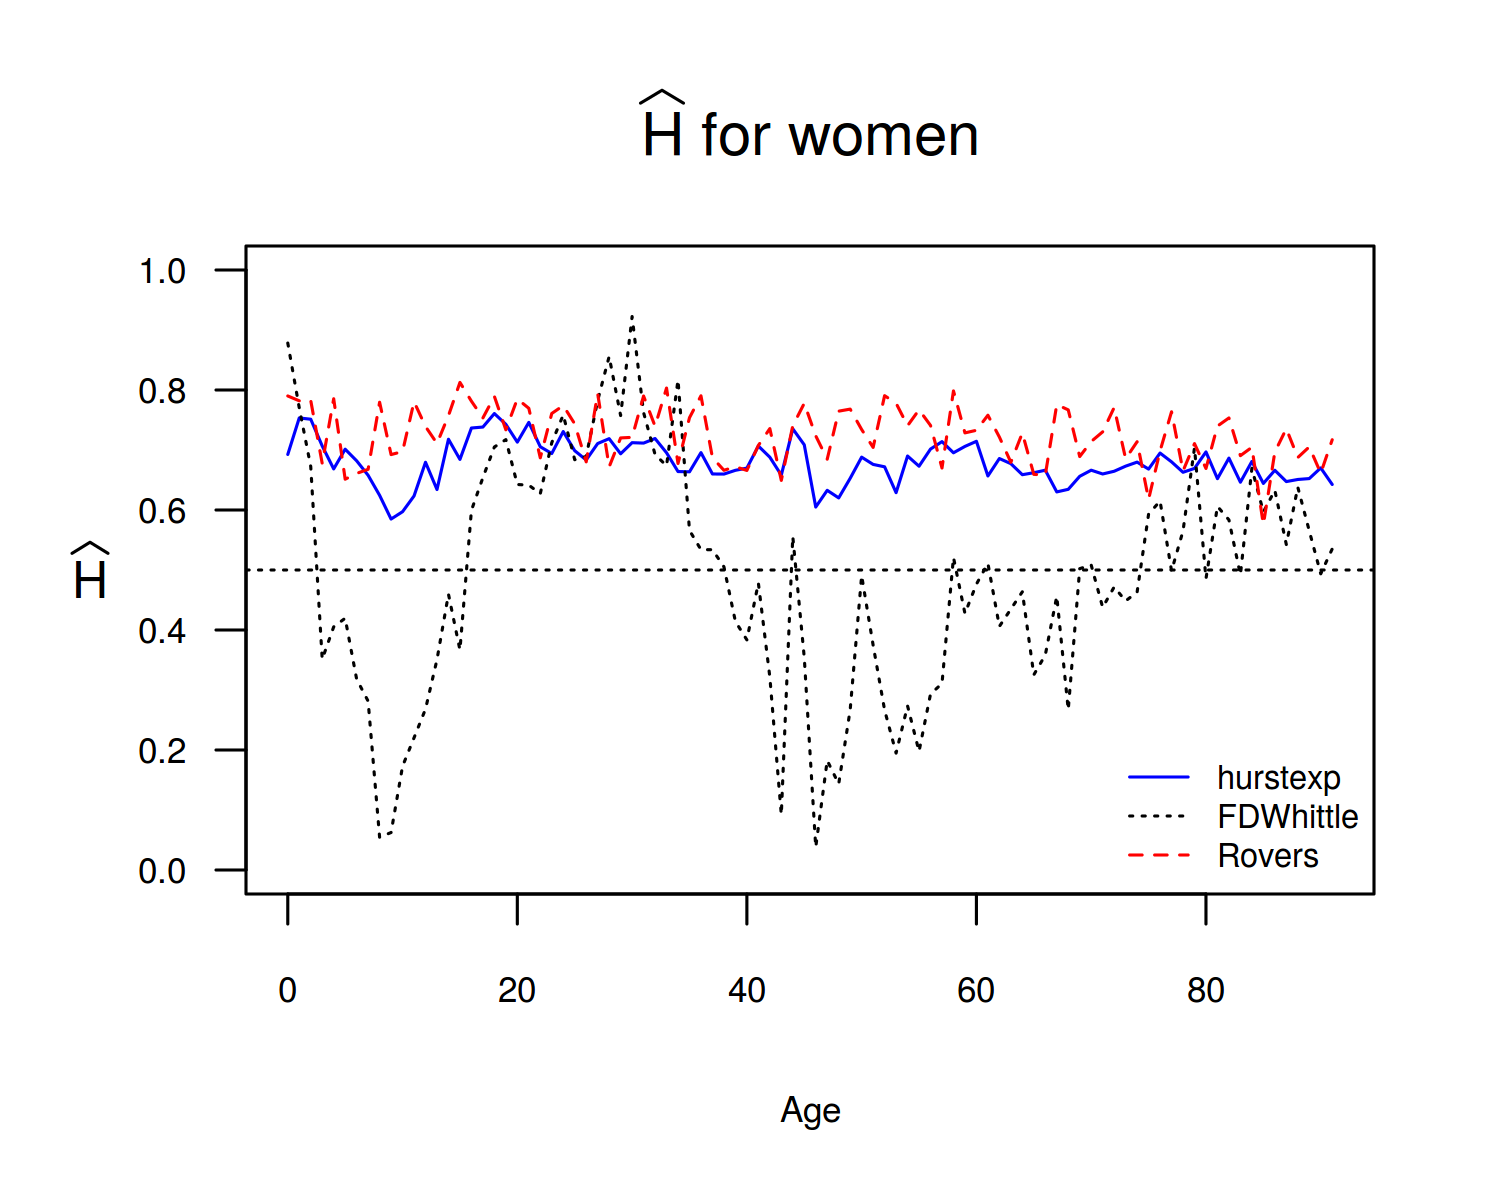
\includegraphics[width = 4.5in,  height=4in]{Hurst-Women.png}
    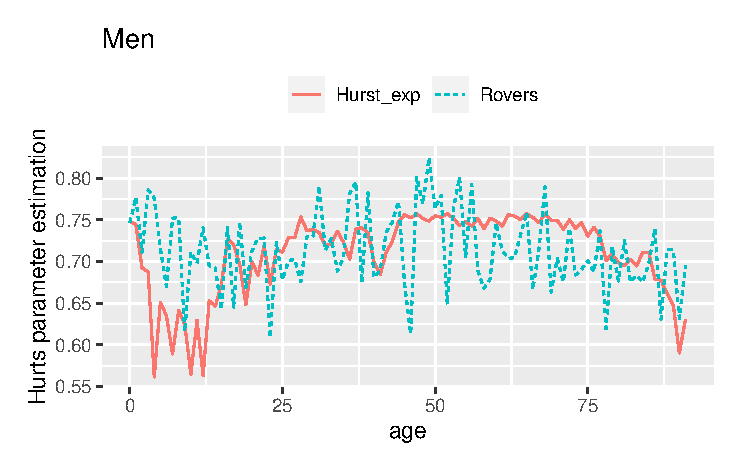
\includegraphics[scale=0.7, keepaspectratio]{Hurst-Men.eps}
    \caption{Estimated Hurst parameter using R-routines.}
    \label{graph-Hurst_Est_Wo}
\end{figure}
\change{change to eps format}


With the rescaled range R/S and R/S  methods we obtain a consistent estimator
for the Hurst
parameter in the sense that they do not present dramatic changes through the
time. Moreover,
the $H$ estimated with these two methods take values in the interval
(0.57,0.80) approximately. This tells us that the data has the long memory
property as
was mentioned in section \ref{fgn}. Same results are obtained for the men and
women.\\


Notice that the estimated parameters for $H$ using Whittle method have high
variation through the time, in opposition to those
obtained with the other two methods so that the estimated
Hurst parameters using this method do not perform well in the simulations.

The high variation on the Hurst estimated values could be explained because
Whittle method uses
the periodogram to estimate $H$ while the other two methods uses the raw data.
The two approaches using Whittle likelihood and raw data are very different and
hence they give very different estimates of $H$. Since rescaled range $R/S$ and
$R/S$  methods have estimated very similar $H$, we decide to use the Hurst
coefficients obtained with the
method of $R/S$ to perform the mortality rates simulations. \\

\begin{figure}[H]
    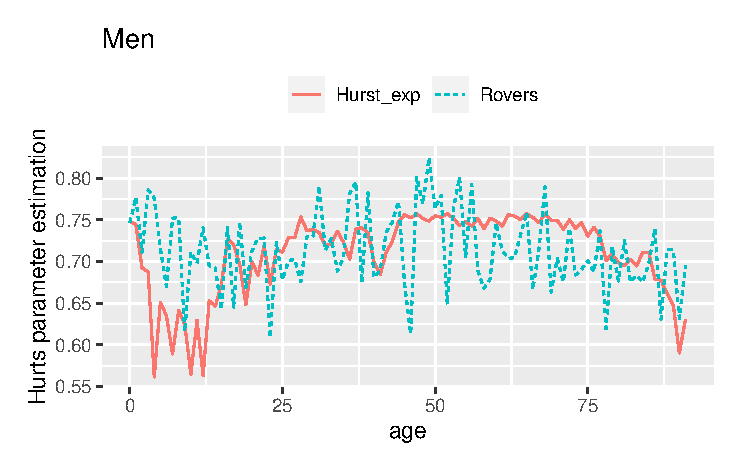
\includegraphics[scale=0.7, keepaspectratio]{Hurst-Men.eps}
    \caption{\bf Estimated Hurst parameter using R-routines.}
    \label{graph-Hurst_Est_Me}
\end{figure}\vspace*{0.1cm}
\change{change to eps format}




\subsection{Results for women}\label{re-wom}

We present the results for 10000 path simulations of the mortality rates for ages:
$0,5,25,50,60,70,80,90$.
We graph the historical mortality rate, the mean of all simulations and the
95\% confidence interval. See figures \ref{graph-simu_FOU1} and
\ref{graph-simu_FOU2}.\\

In general, for all ages, the model is well fitted, in particular, after the
80's. Nevertheless, there are some time periods where the model is not
so good as we want to. For instance, the model underestimates the mortality
rate for women age 0 during the period of 50s to 80s and for women age 50, 60,
80 and 90 during
60s to 80s approximately. Moreover, it also overestimates the mortality rate for
women age 25 during the period of 50s to 80s.


\begin{figure}[t]
    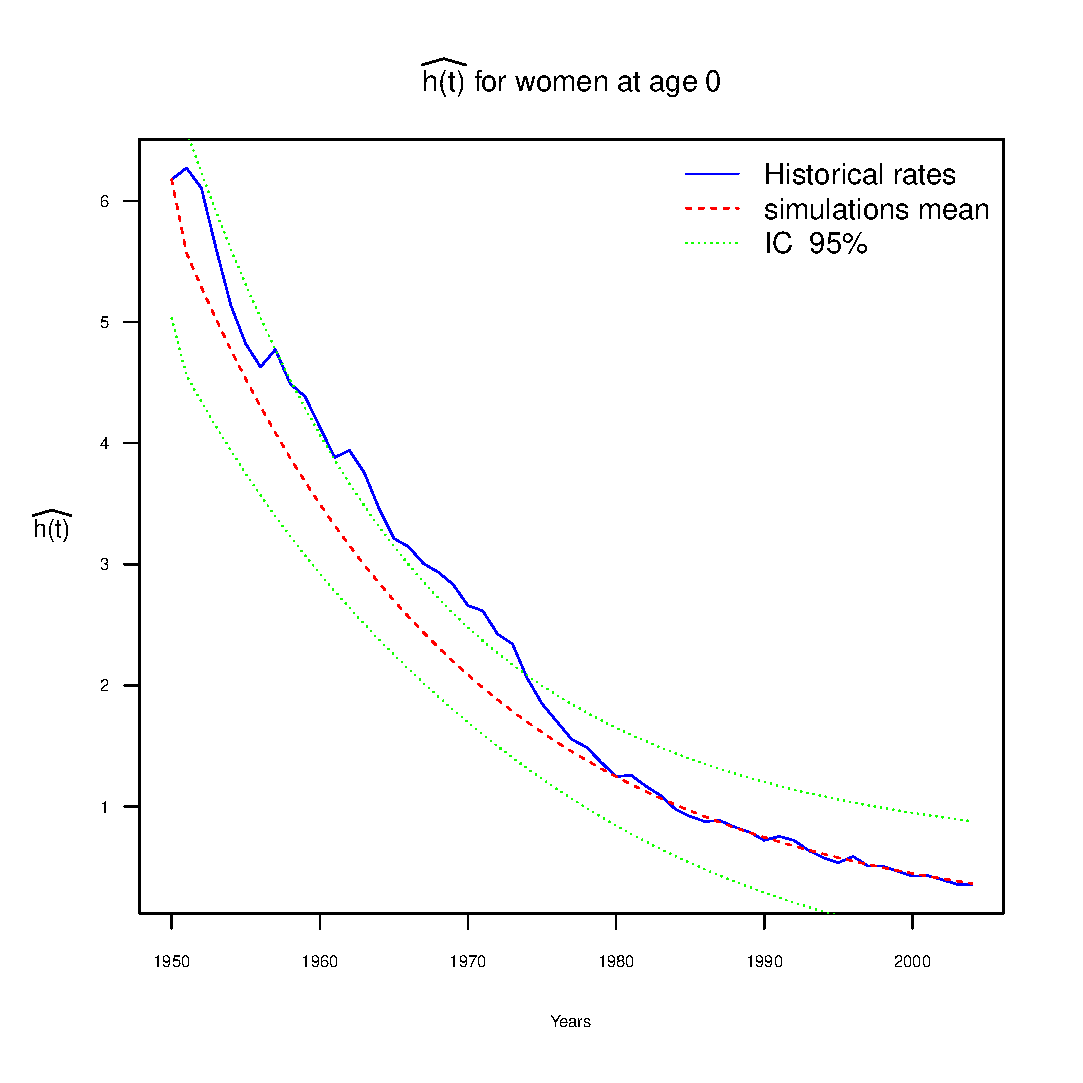
\includegraphics[scale= 0.5, keepaspectratio]{PlotWomen0.eps}
    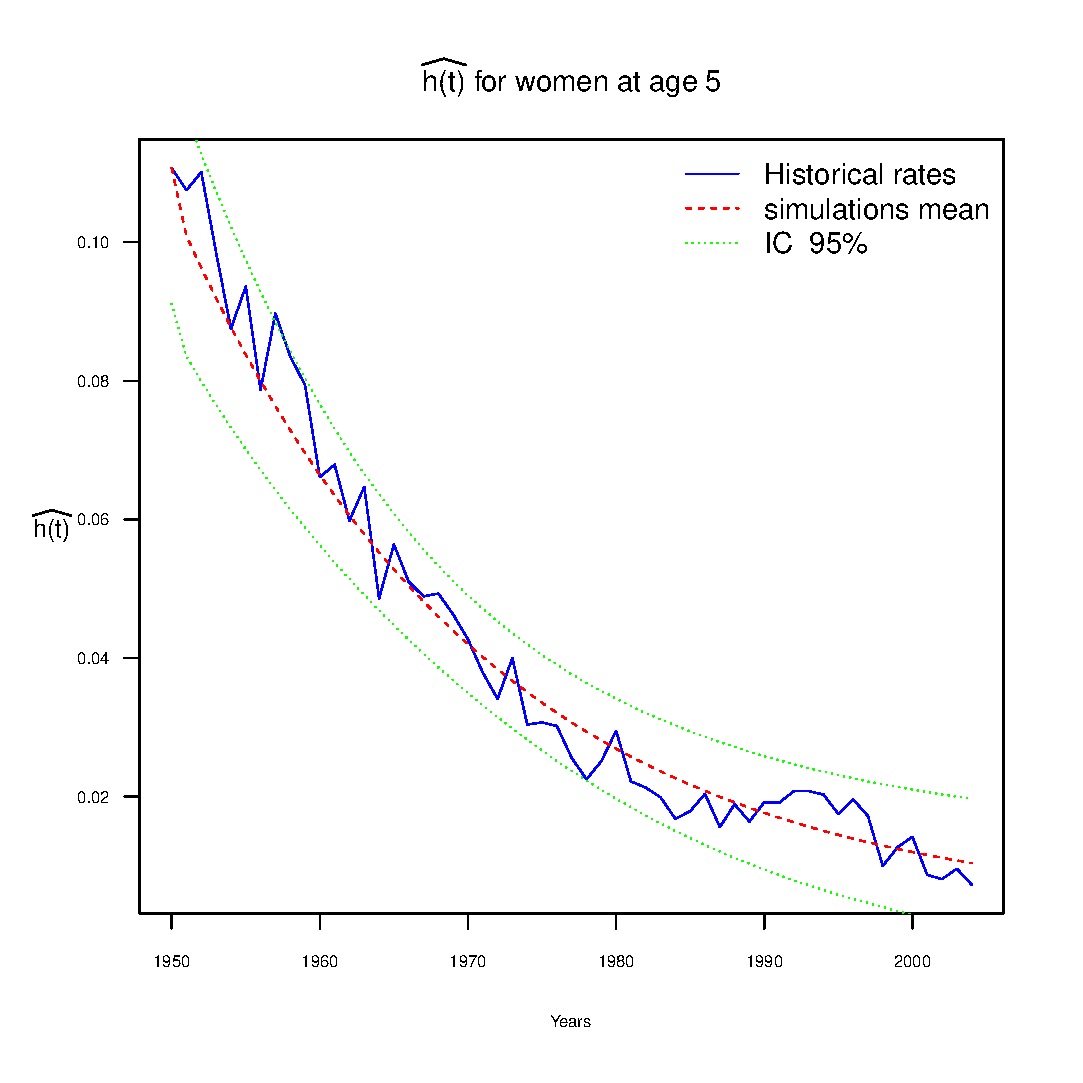
\includegraphics[width = 2.85in]{PlotWomen5.eps}
    \includegraphics[width = 2.85in]{PlotWomen25.eps}
    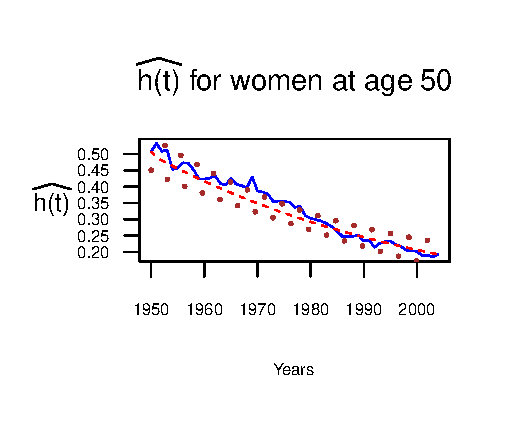
\includegraphics[width = 2.85in]{PlotWomen50.eps}
    \caption{Simulations for the rate mortality with the fOU model: ages
    $0,5,25,50$ and $N=10000$.}
    \label{graph-simu_FOU1}
\end{figure}

%From the data we have noticed that, for ages between 20 to 35 approximately
%(in the beginning of the 90's) the phenomena of AIDS has made a little
%increase
%in the rates mortality; however, the model captures this circumstance well,
%since the estimation still remains inside
%the confidence intervals. We believed that in order  to compensate this
%variation, the model overestimates mortality rates
% for the period between late 50's and first 70's. \\


For older ages (see figure \ref{graph-simu_FOU2}) we observe that for ages 60
and 70 the estimation is well fitted trough the years. We notice that
predicted rates are not so far away and that the historical rates are inside
the confidence interval. For the very oldest ages the estimation is not so good
as for earlier ages. The main difference is in 50's when the absolute number of
living persons arriving to those ages were small so that the variability of the
estimates is larger. \\

All these suggest that a better model could include a short and a long-term
memory process, so that the model could help us to control the short-term
variations in a better way.

\begin{figure}[htb]
    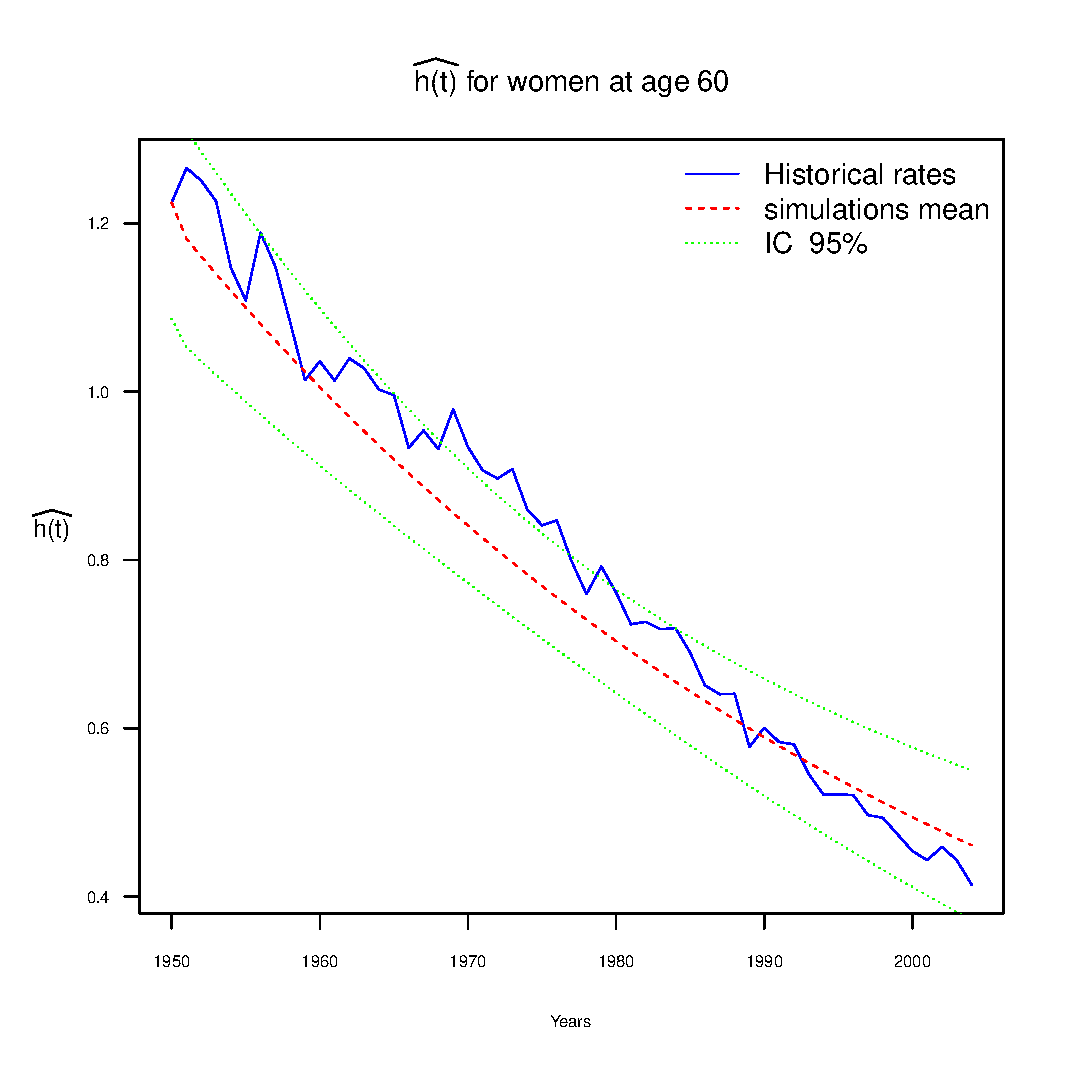
\includegraphics[width = 2.85in]{PlotWomen60.eps}
    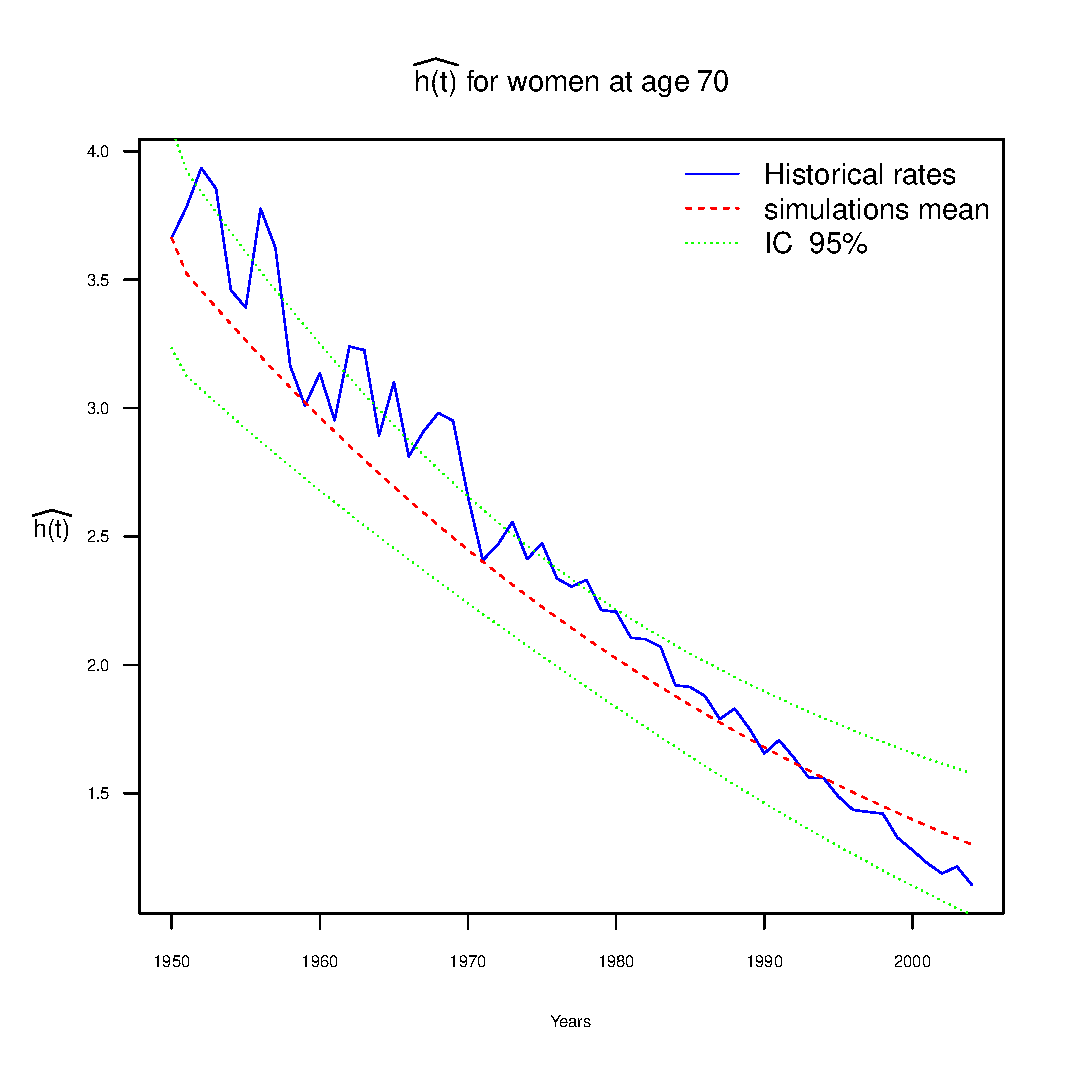
\includegraphics[width = 2.85in]{PlotWomen70.eps}
    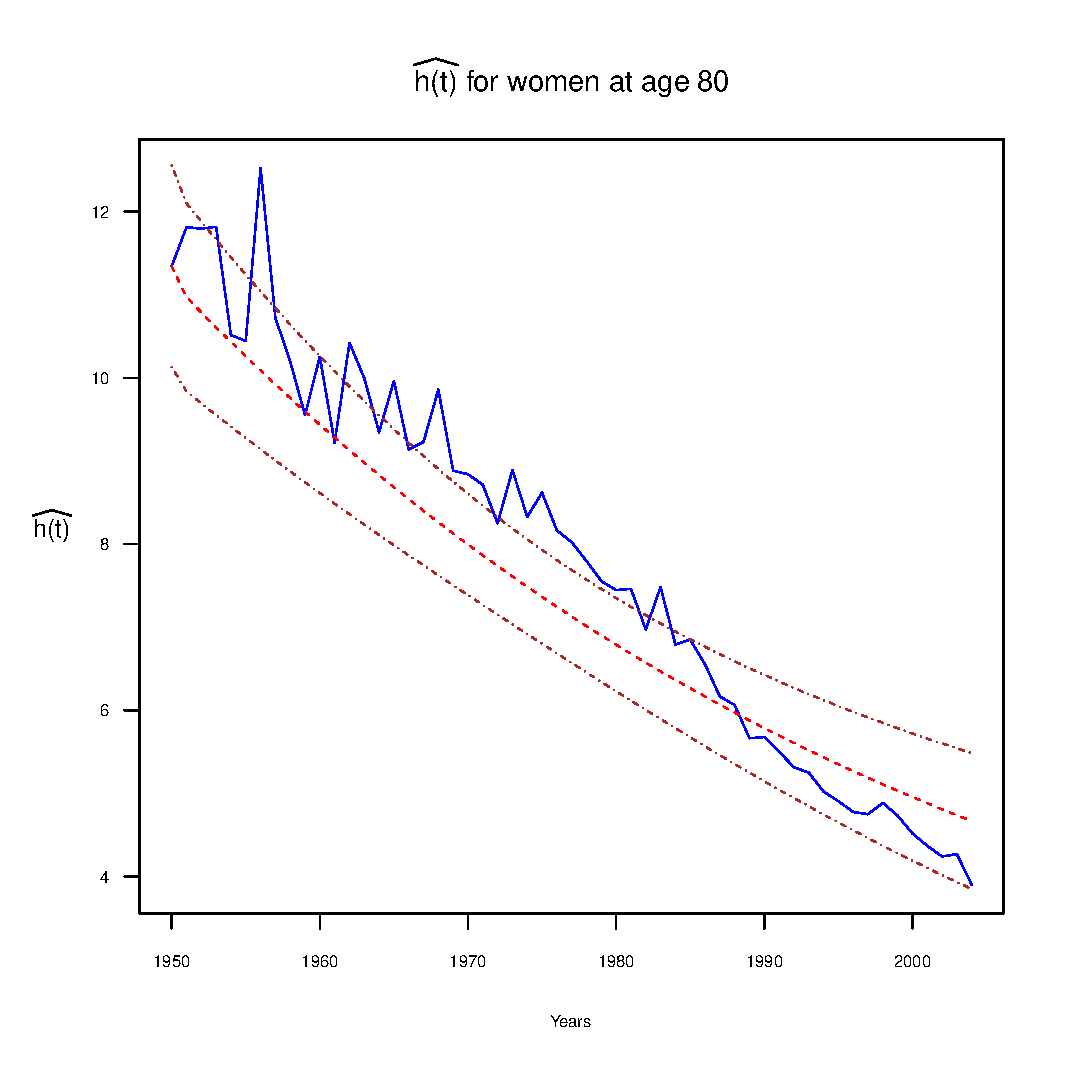
\includegraphics[width = 2.85in]{PlotWomen80.eps}
    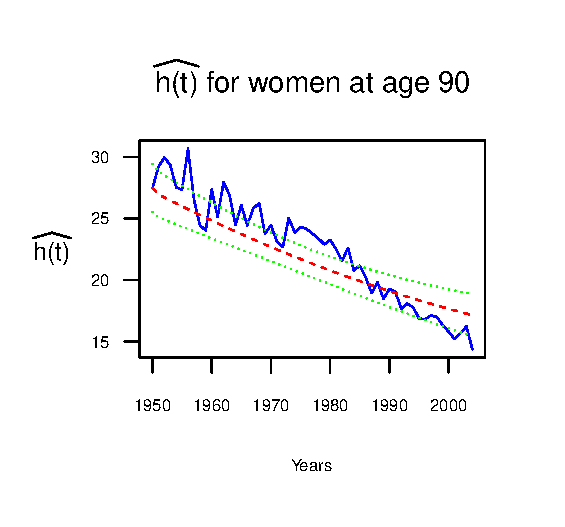
\includegraphics[width = 2.85in]{PlotWomen90.eps}
    \caption{\bf Simulations for the rate mortality with the fOU model: ages
    $60,70,80,90$ and $N=10000$.}
    \label{graph-simu_FOU2}
\end{figure}\vspace*{0.1cm}


\subsection{Results for men}\label{re-men}

As in the case for women, we present results for 10000 simulations of the
mortality rates for ages: $0,5,25,50,60,70,80,90$.
We graph the historical rate mortality, the mean of all simulations and the
95.5\% confidence interval. See figures \ref{graph-simu_FOU3} and
\ref{graph-simu_FOU4}.\\



\begin{figure}[H]
    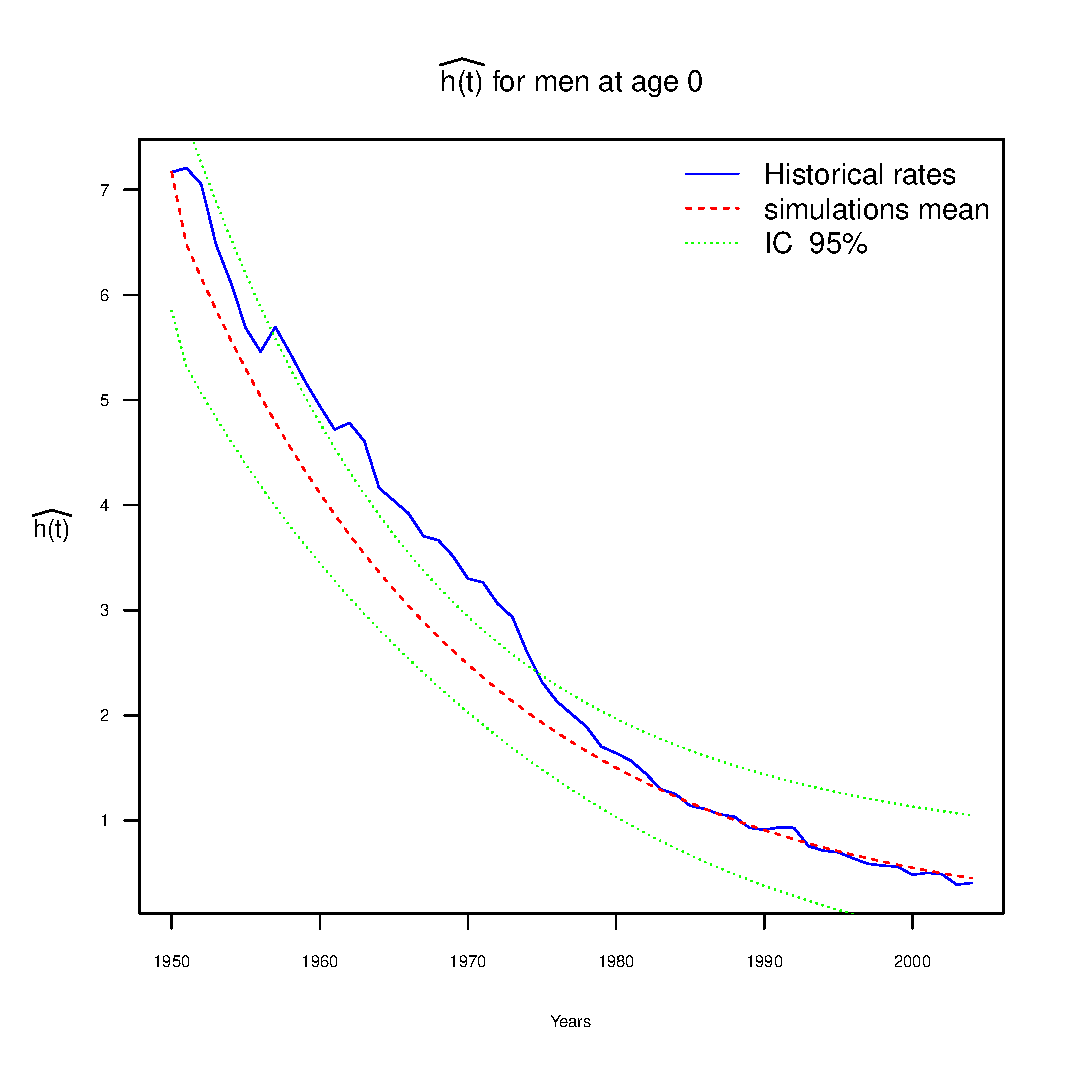
\includegraphics[width = 2.85in]{PlotMen0.eps}
    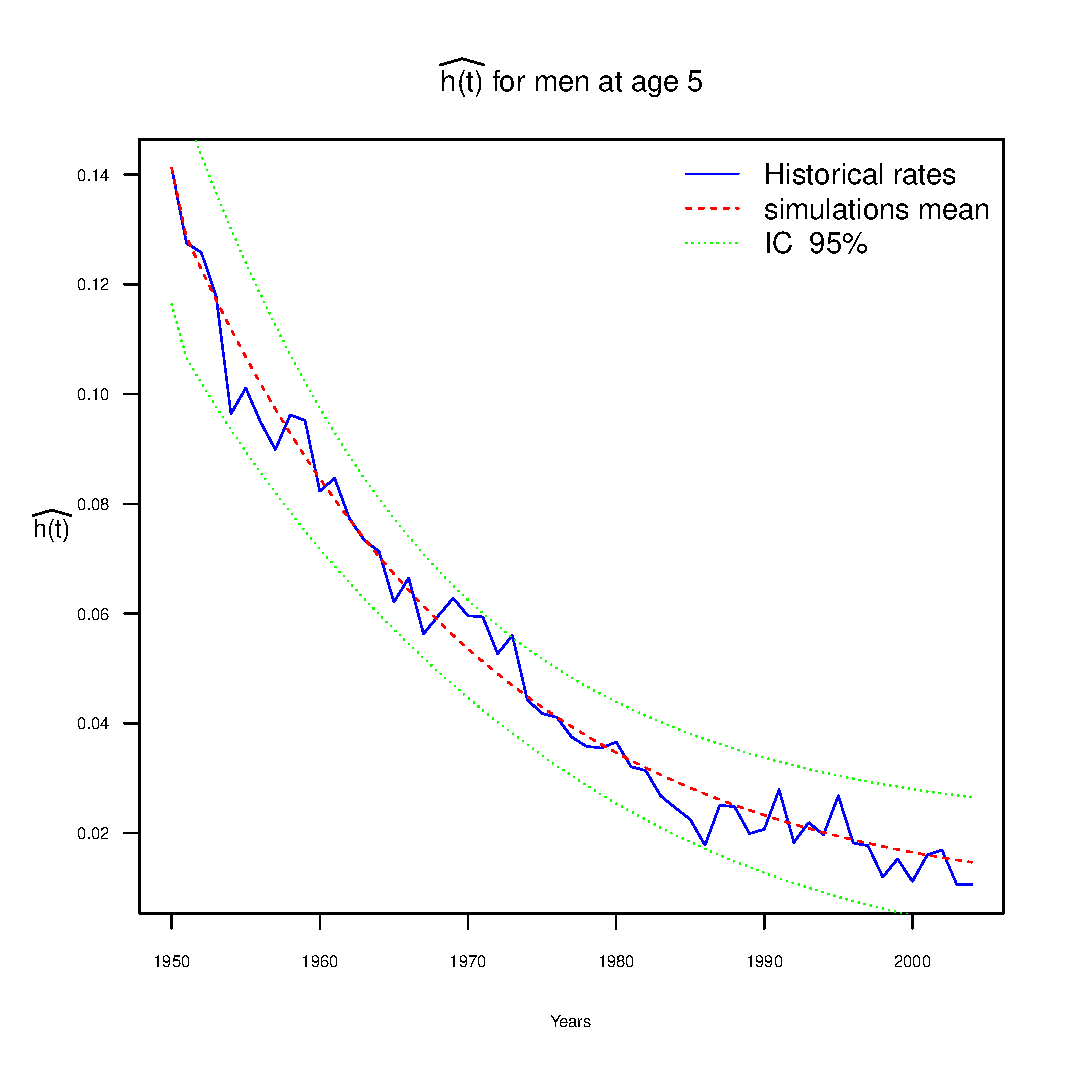
\includegraphics[width = 2.85in]{PlotMen5.eps}
    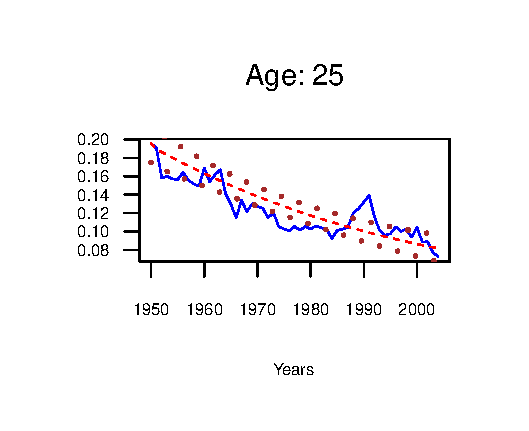
\includegraphics[width = 2.85in]{PlotMen25.eps}
    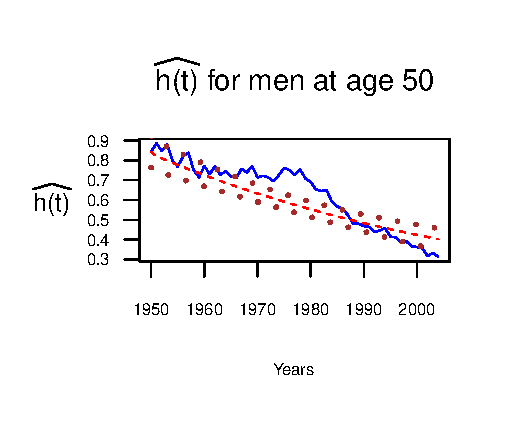
\includegraphics[width = 2.85in]{PlotMen50.eps}
    \caption{\bf Simulations for the rate mortality with the fOU model: ages
    $0,5$ and $N=10000$.}
    \label{graph-simu_FOU3}
\end{figure}\vspace*{0.1cm}

As in the case for women, the proposed model for men is well fitted.
%The AIDS pandemic is also noticed for ages between 25 to 35 and
%it generates an increase in the rates mortality for these ages; As a matter of
%fact, this increase is heavier
We observe an increase in the rates mortality at ages between 25 to 35, this
caused a overestimation in the first 35 years and latter a underestimation
of the mortality rates. As was mentioned before, if we include in the model a
short-term process,  we believe the model could be better fitted. The main
example  of a short-term process to try is a AR$(p)$ with $p\le 2$ or $3$.

\begin{figure}[H]
    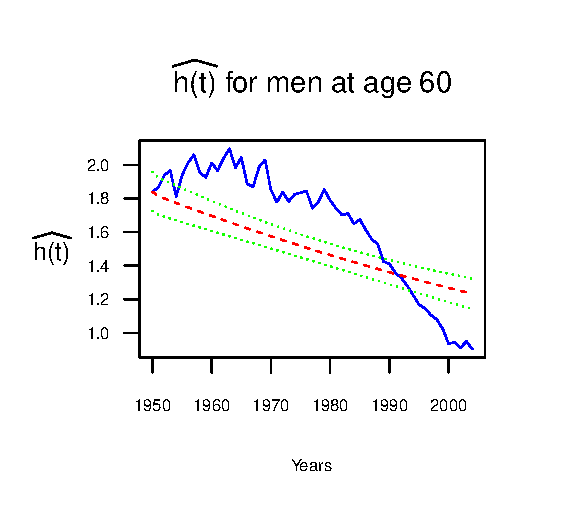
\includegraphics[width = 2.85in]{PlotMen60.eps}
    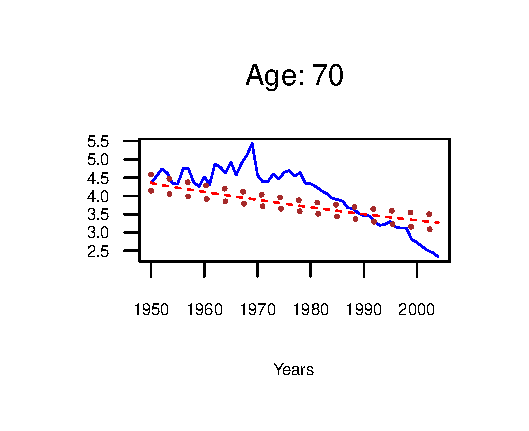
\includegraphics[width = 2.85in]{PlotMen70.eps}
    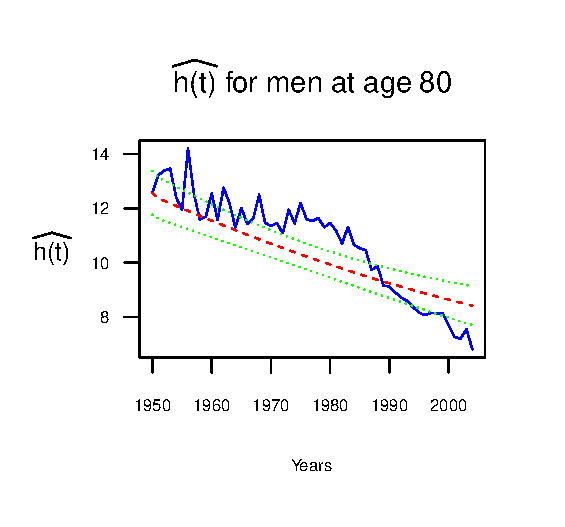
\includegraphics[width = 2.85in]{PlotMen80.eps}
    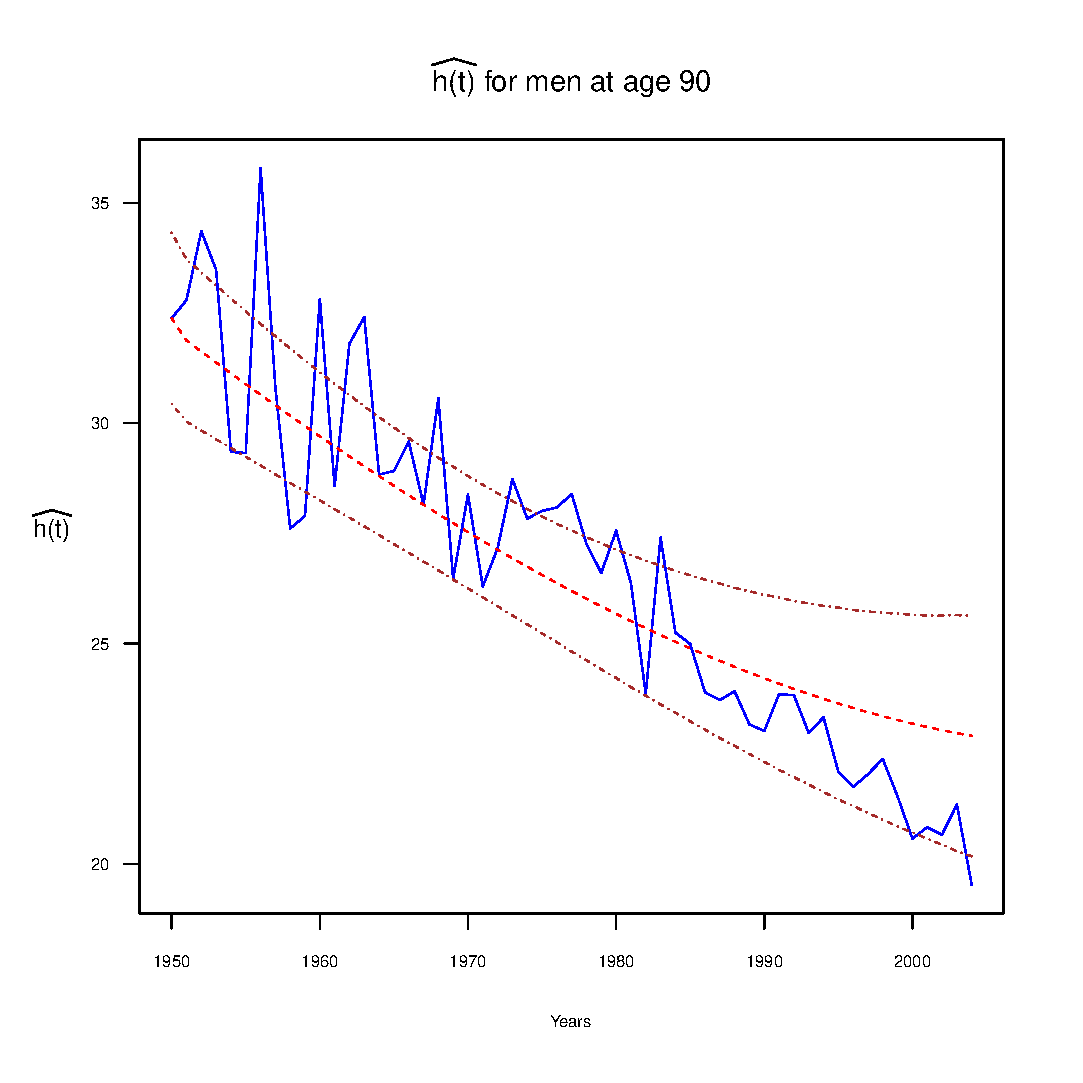
\includegraphics[width = 2.85in]{PlotMen90.eps}
    \caption{\bf Simulations for the rate mortality with the fOU model: ages
    $60,70,80,90$ and $N=10000$.}
    \label{graph-simu_FOU4}
\end{figure}\vspace*{0.1cm}

For older ages, we observed that the data is irregular, so it is necessary to
use a more complex model to
fit this data.

\section{Forecast}

When we use our model to forecast and compare with the real data between the
years 2005 to 2014. In general, from our results we observe that the forecast
for women are good for almost all ages we tested. For men the variability of
the results is strong and the behavior of the forecast is in general not good
as those for women; for instance for ages smaller than 10 the results are quite
similar than for women, even for ages between 10 and 45 it is possible to
consider the results just good. However, for ages greater than 50, the results
are not good, in fact, for older ages the results are bad: the model
overstimate the mortality rates.

We present the results in the figures \ref{graph-graph-forecast_women_FOU1} for
women at ages $0,25,50,90$. For men we present more ages to ilustrate that the
results are bad as the ages increases. see figures
\ref{graph-forecast_men_FOU1} and \ref{graph-forecast_men_FOU2} at ages
$0,25,50,90$.

\begin{figure}[H]
    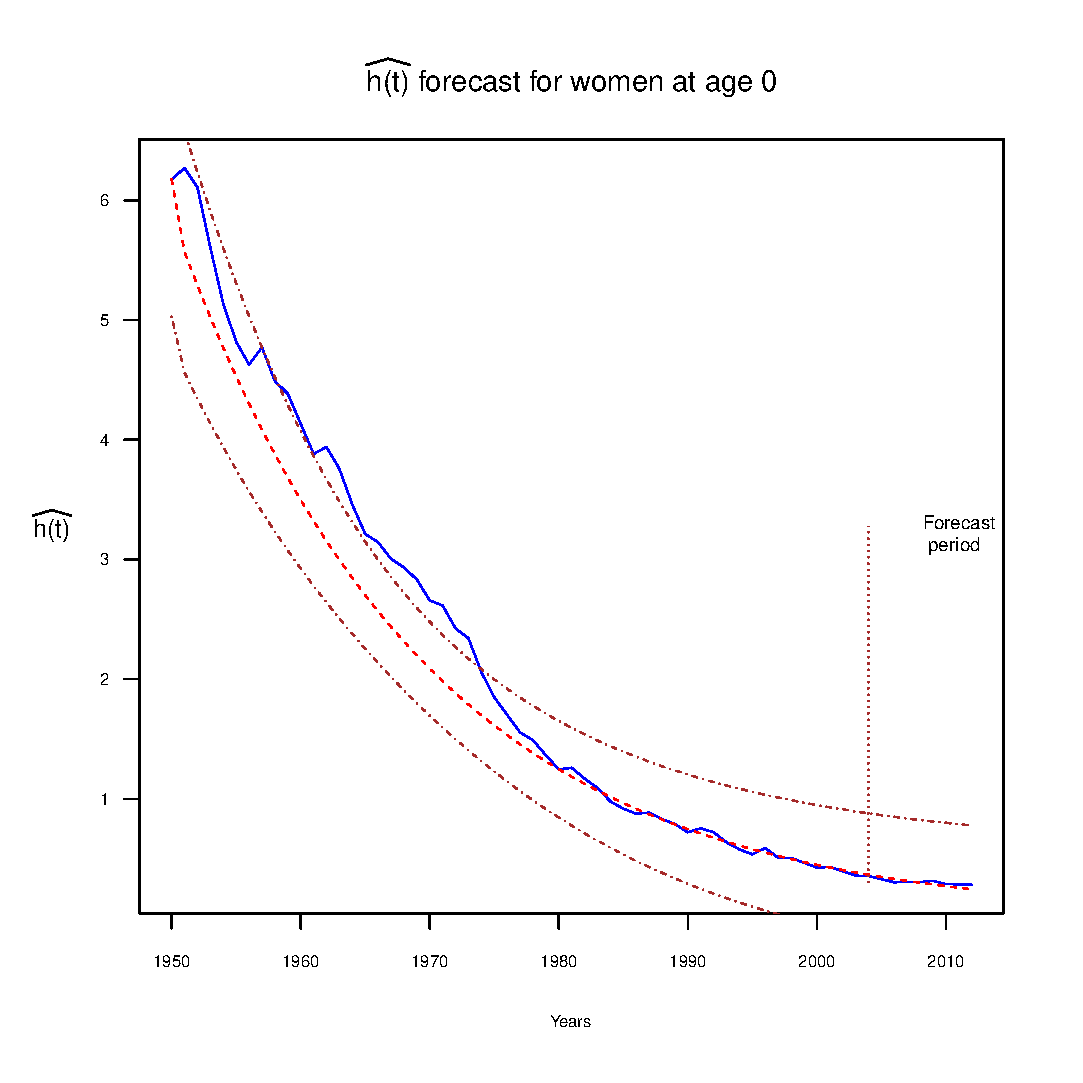
\includegraphics[width = 2.85in]{PlotWomenForecast0.eps}
    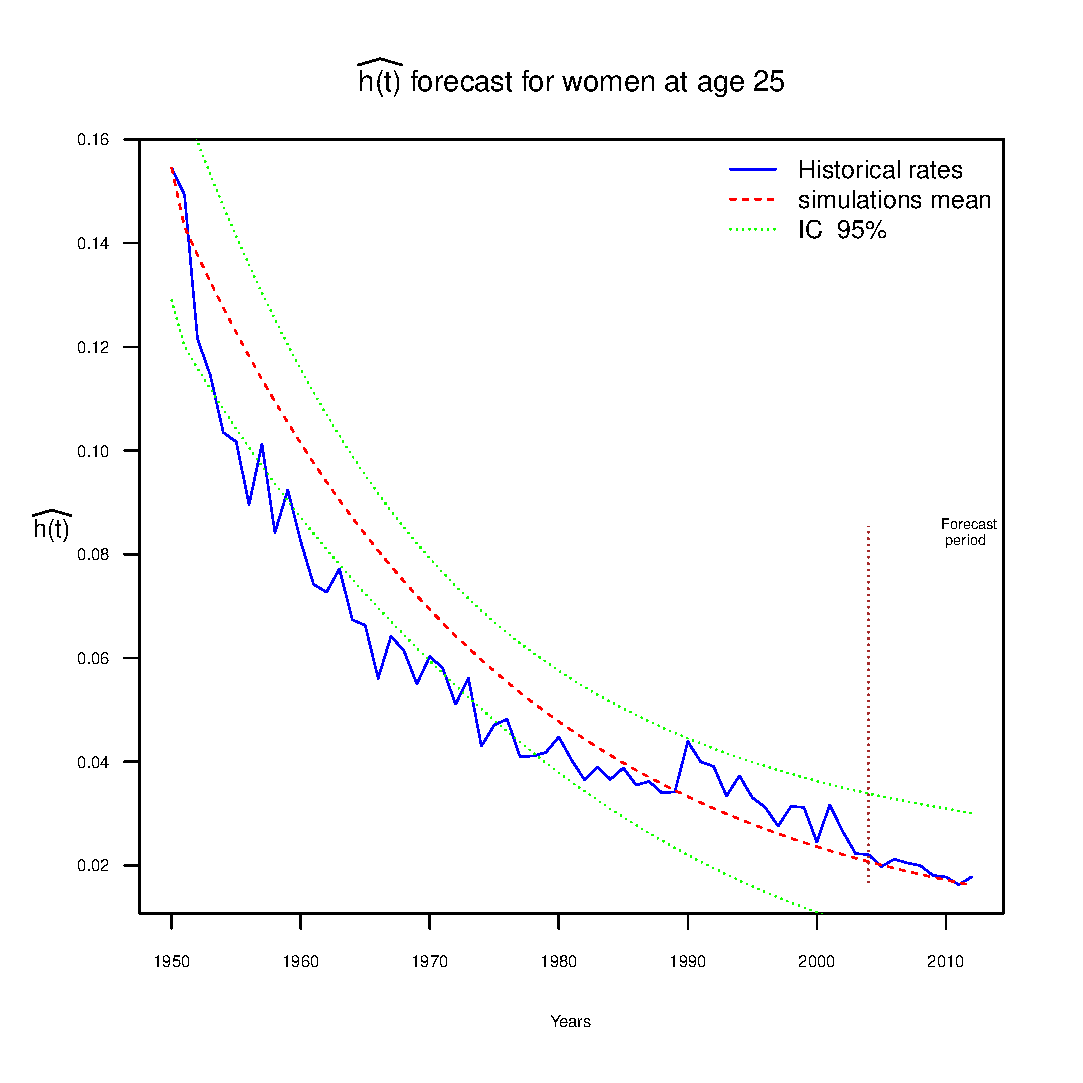
\includegraphics[width = 2.85in]{PlotWomenForecast25.eps}
    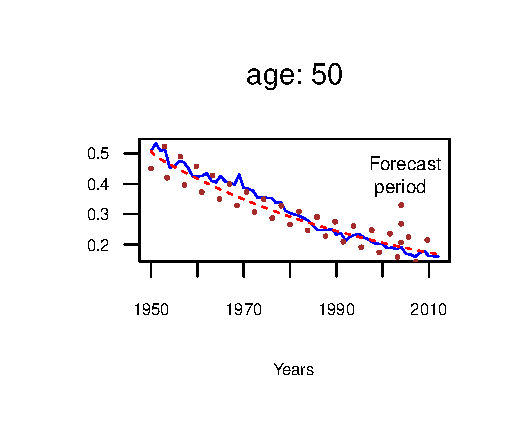
\includegraphics[width = 2.85in]{PlotWomenForecast50.eps}
    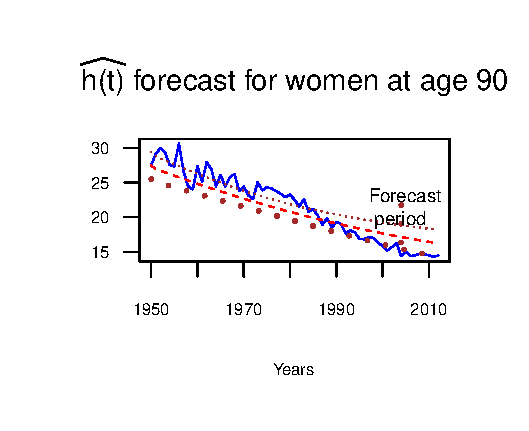
\includegraphics[width = 2.85in]{PlotWomenForecast90.eps}
    \caption{Forecast for the rate mortality with the fOU model. Women at ages
    $0,25,50,90$.}
    \label{graph-graph-forecast_women_FOU1}
\end{figure}\vspace*{0.1cm}




\begin{figure}[H]
    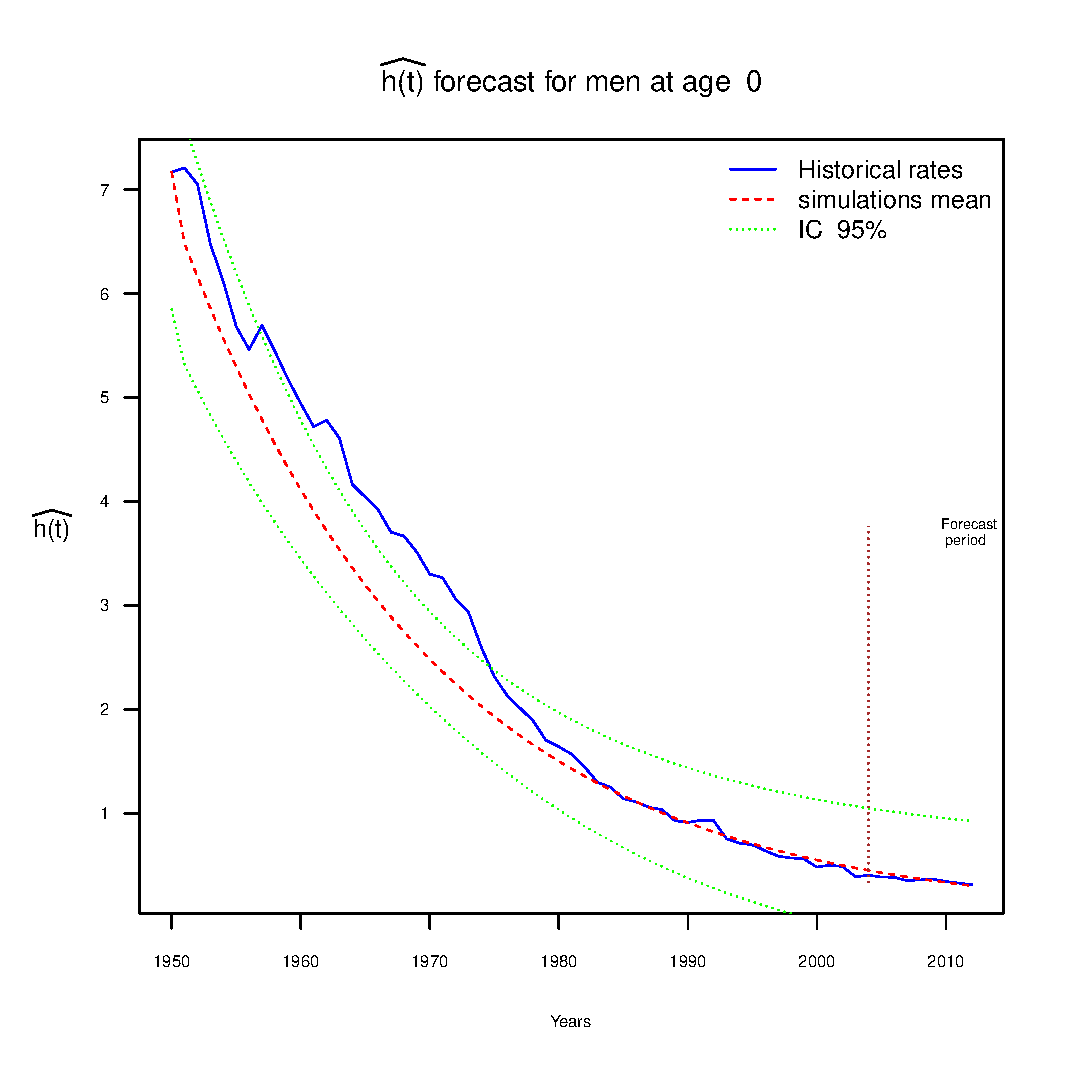
\includegraphics[width = 2.85in]{PlotMenForecast0.eps}
    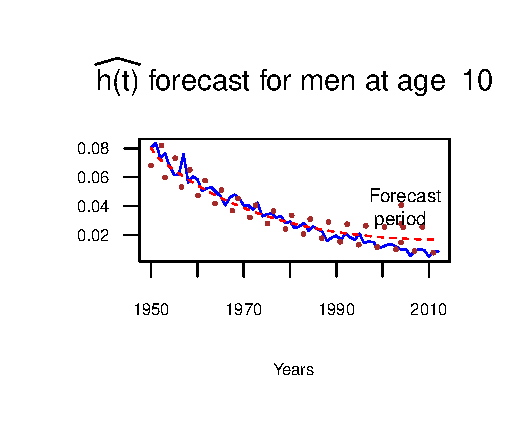
\includegraphics[width = 2.85in]{PlotMenForecast10.eps}
    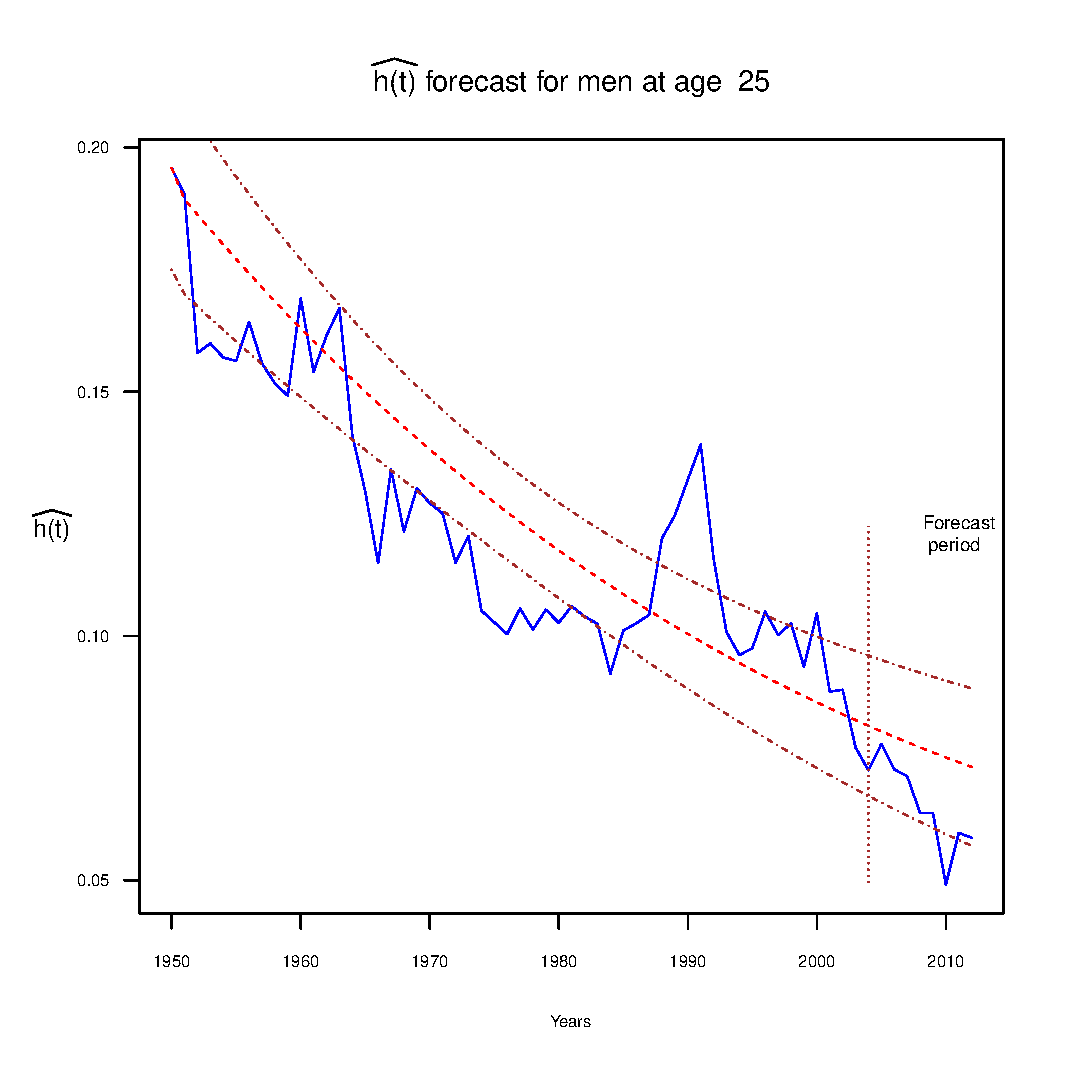
\includegraphics[width = 2.85in]{PlotMenForecast25.eps}
    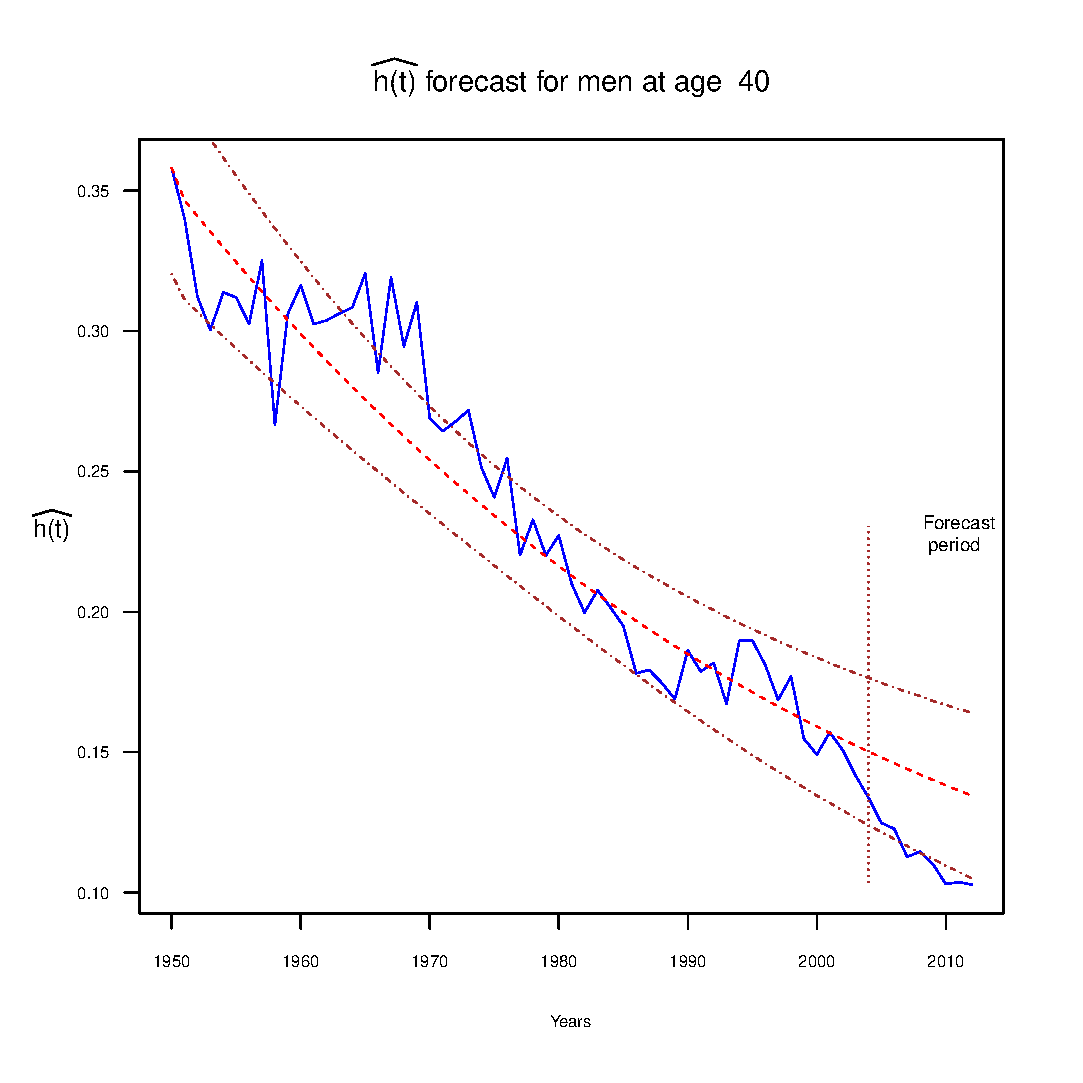
\includegraphics[width = 2.85in]{PlotMenForecast40.eps}
    \caption{Forecast for the rate mortality with the fOU model. Men at ages
    $0,10,25,40$.}
    \label{graph-forecast_men_FOU1}
\end{figure}\vspace*{0.1cm}



\begin{figure}[H]
    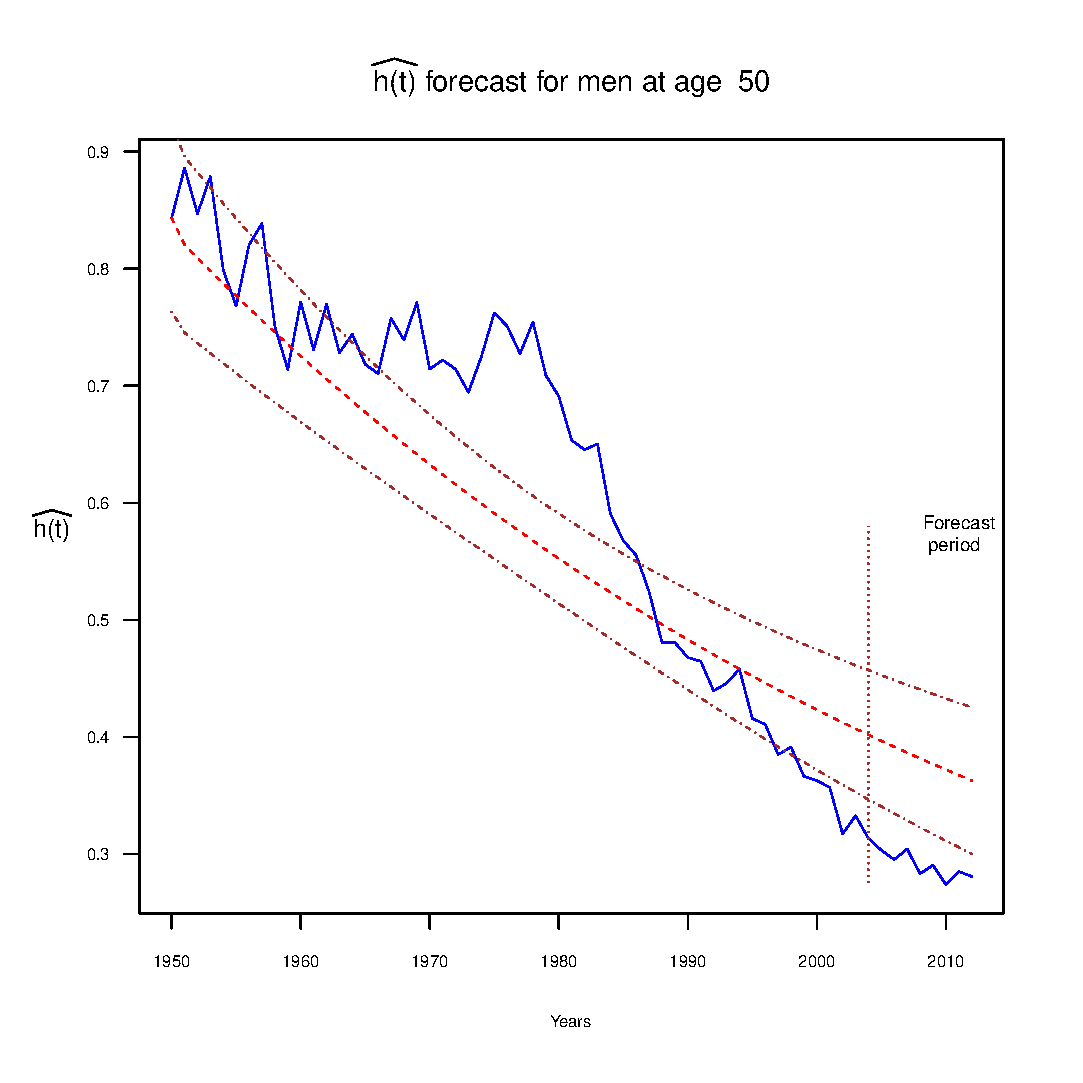
\includegraphics[width = 2.85in]{PlotMenForecast50.eps}
    \includegraphics[width = 2.85in]{PlotMenForecast60.eps}
    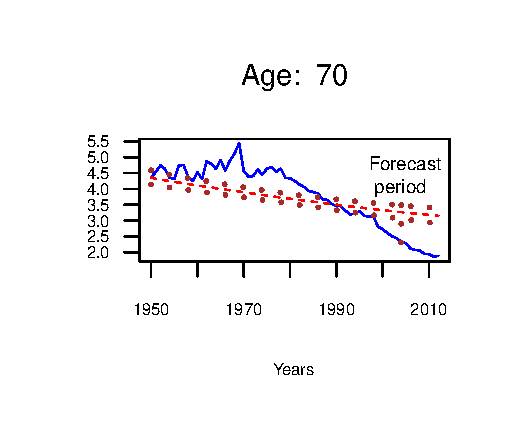
\includegraphics[width = 2.85in]{PlotMenForecast70.eps}
    \includegraphics[width = 2.85in]{PlotMenForecast90.eps}
    \caption{Forecast for the rate mortality with the fOU model. Men at ages
    $50,60,70,90$.}
    \label{graph-forecast_men_FOU2}
\end{figure}\vspace*{0.1cm}


\section{Conclusions}\label{sec:Conclutions}

We have applied our proposed model to the Italian mortality rates with a
geometric-type fractional Ornstein-Uhlenbeck process. Our
main hypothesis was that, for a fixed age, the mortality rates changes through
the time slowly, so that a stochastic differential equations
that captures the long-range dependence could be a good model. We have used a
stochastic differential equation with a fractional Brownian motion as a driven
noise with $H\in (0.5,1)$ in order to satisfy the long-range dependence
property. With the data we have fixed the Hurst coefficient and we have
confirmed our hypothesis since
we have found that the estimated Hurst, for all ages, is in $(0.58,0.8)$.  \\



Notice that we have consider a more general model that the one used in
\cite{gi-or-be}. This is because we have included the possibility that the
Hurst parameter could be equal to $1/2$, which is the case when the fractional
Brownian motion becomes a standard Brownian motion. Therefore,
when $H=1/2$ we recover the  Giacometti, Ortobelli and Bertocchi model.\\




% FGN with  single parameter $H$ is a simplified model of reality. Therefore,
% it may be not appropriate for some phenomena, even though it is much more
%consistent with reality than the AR and ARMA process.
% A generalized and comprehensive family of processes, which can include a
%larger number of parameters and incorporates both the
% FGN and the ARMA processes, has been studied by Koutsoyiannis \cite{kou}. One
%possible generalization
% of the ARMA process is the FARIMA process, which is a long memory process
% (see, for instance, section 5.2 in \cite{sh-st}).



The model is, specially for women, well behaved. For men at some ages we found
some shortcomings that suggest the use of more terms in order to improve the model. 
From this results, and in opposition of the European normative on insurance that does not discriminate by gender, we conclude from our model, applied to the Italian case, that modelling the mortality by gender could improve the risk management of the insurance companies.\\


The long-range dependence model proposed in this paper is good
enough to reproduce the mortality rates. If we add some extra terms to make it
more flexible to reproduce the cases where the mortality rates have more
variations then it will generate a more accurate model. We are starting to work
on this extension of the model. Moreover, a multiplicative noise model will be
the subject of a future research.\\



\bibliography{references.bib}{}
\bibliographystyle{rss}
% \begin{thebibliography}{99}

%     \bibitem{be-ye-fe-gh} J. Beran, Y. Feng, S. Ghosh, R. Kulik: Long-Memory
%     Processes. Probabilistic Properties and Statistical Methods.
%     Springer. (2013)

%     \bibitem{br-ia} A. Brouste, S. M. Iacus: {\it  Parameter estimation for the
%     discretely observed fractional Ornstein-Uhlenbeck process
%         and the Yuima R package}. Computational Statistics August 2013, Volume
%         28, Issue 4, pp 1529-1547. (2013).
%     \bibitem{ch-ka-ma} P. Cheridito, H. Kawaguchi, M. Maejima {\it Fractional
%     Ornstein-Uhlenbeck processes}. Electron J Probab
%     8(3):1-14, (2003).

%     \bibitem{de} I. Daubechies: Ten Lectures on Wavelets, SIAM (1992)

%     \bibitem{du-no} R.M. Dudley, R. Norvai\v{s}a: Concrete functional calculus,
%     in: Springer Monographs in Mathematics, Springer, New
%     York, 2011.

%     \bibitem{gi-or-be} R. Giacometti, S. Ortobelli, M. Bertocchi:{\it A
%     Stochastic Model for Mortality Rate on Italian Data}
%     Journal of Optimization Theory and Applications 149 (1), 216-228. (2011).


%     \bibitem{hu-nu} Y. Hu, D. Nualart : {\it Parameter estimation for
%     fractional Ornstein–Uhlenbeck processes}. Stat Probab
%     Lett 80(11–12):1030–1038. (2010).


%     \bibitem{hu} H. E. Hurst: {\it Long-term storage capacity in reservoirs}.
%     Trans. Amer. Soc. Civil Eng. 116, 400-410. (1951).
%     \bibitem{is-la} J. Istas, G. Lang : {\it Quadratic variations and
%     estimation of the local Hölder index of a Gaussian process}.
%     Annales de l’Institut Henri Poincaré 23(4):407–436. (1997).
%     \bibitem{je-lu-vi} P. Jevtić, E. Luciano, E. Vigna: {\it Mortality surface
%     by means of continuous time cohort models}.
%     Insurance:Mathematics and Economics. Volume 53, Issue 1, July 2013, Pages
%     122–133. (2013).


%     \bibitem{kl-pl} P. E. Kloeden, E. Platen: Numerical Solution of Stochastic
%     Differential Equations. Stochastic
%     Modelling and Applied Probability, Vol. 23, Springer (1992)
%     \bibitem{ko}  A. N. Kolmogorov: {\it Wienersche Spiralen und einige andere
%     interessante Kurven  im
%         Hilbertschen Raum}. C. R. (Doklady) Acad. URSS (N.S.) 26, 115-118.
%         (1940).
%     \bibitem{kou} D. Koutsoyiannis: {\it The Hurst phenomenon and fractional
%     Gaussian noise made easy}.
%     Hydrological Sciences Journal des Sciences Hydrologiques, 47(4). August
%     (2002)
%     \bibitem{ku-mi} K. Kubilius, Y. S. Mishura: {\it The rate of convergence of
%     Hurst index estimate for the stochastic differential equation}
%     Stochastic Processes and their Applications. Vol. 122, Issue 11,
%     3718–3739. (2012)
%     \bibitem{lo} A. W. Lo: {\it Long-Term Memory in Stock Market Prices}
%     Econometrica Vol. 59, No. 5 (Sep., 1991), pp. 1279-1313. (1991).
%     \bibitem{ma-va}  B. B. Mandelbrot, J. W. Van Ness: {\it Fractional Brownian
%     motions, fractional noises and
%         applications}. SIAM Review 10, 422-437. (1968).
%     \bibitem{mik} T. Mikosch : Elementary Stochastic Calculus With Finance in
%     View. Advanced Series on Statistical Science and Applied
%     Probability, Vol 6. World Scientific Publishing (1999)
%     \bibitem{mi-pr}  M.A. Milevsky, S.D. Promislow: {\it Mortality derivatives
%     and the option to annuitise}. Insur. Math.
%     Econ. 29, 299–318 (2001)
%     \bibitem{mi}  Y. S. Mishura: Stochastic Calculus for Fractional Brownian
%     Motion and Related Processes.
%     Springer, (2008).

%     \bibitem{ne-ti} A. Neuenkirch, S. Tindel: {\it A least square-type
%     procedure for parameter estimation in stochastic differential
%         equations with additive fractional noise}. Stat Inference Stoch
%         Process, vol. 17, 99–120, (2014).


%     \bibitem{nu} D. Nualart: {\it Fractional Brownian motion: stochastic
%     calculus and applications }
%     Proceedings of the International Congress of Mathematicians, Madrid, Spain,
%     (2006)
%     \bibitem{ok} B.K. \"Oksendal: Stochastic Differential Equations: An
%     Introduction with Applications. Berlin: Springer.  (2010).

%     \bibitem{pa-etal} C. Park, F. Hernandez-Campos, L. Long, J. Marron, J.
%     Park, V. Pipiras, F. Smith, R. Smith, M. Trovero, Z. Zhu:
%     {\it Long range dependence analysis of internet traffic}. J. Appl. Stat.
%     38(7), 1407-1433 (2011)
%     \bibitem{priestley} M. Priestley Spectral Analysis and Time Series.
%     Academic Press (1982)
%     \bibitem{ra} B. L. S. Prakasa Rao: Statistical Inference for Fractional
%     Diffusion Processes. Wiley Series in Probability and Statistics.
%     (2010)
%     \bibitem{ro-le} A. Rossa, L. Socha: {\it Proposition of a Hybrid Stochastic
%     Lee-Carter Mortality Model}. Advances in Methodology \&
%     Statistics/Metodoloski zvezki 10.1 (2013).


%     \bibitem{sh-st} R. H. Shumway, D. S. Stoffer: {\it Time Series Analysis and
%     Its Applications: With R Examples}.
%     Springer Texts in Statistics. 3rd. ed. (2011).
%     \bibitem{yo}  L.C. Young: {\it An inequality of the H\"older type,
%     connected with Stieltjes integration}, Acta Mathematica 67
%     251–282. (1936).
%     \bibitem{we} R. Weron:{\it Estimating long-range dependence: finite sample
%     properties and confidence intervals}.
%     Physica A 312 (2002) 285 - 299

%     \bibitem{ye-etal} F. Yerlikaya-Ozkurt, C. Vardar-Acar, Y. Yolcu-Okur, G.-W.
%     Weber:
%     {\it Estimation of the Hurst parameter for fractional Brownian motion using
%     the CMARS method}.
%     J. Comput. Appl. Math., 259, pp. 843-850.  (2014).

%     \bibitem{ze-ch-ya} C: Zeng, Y. Q. Chen, Q. Yang: {\it The fBm-driven
%     Ornstein-Uhlenbeck process: Probability density function and
%         anomalous diffusion}. Fractional Calculus and Applied Analysis
%         September 2012, Volume 15, Issue 3, pp 479-492. (2012).


% \end{thebibliography}
\end{document}
